\documentclass[journal]{IEEEtran}

\usepackage{amsmath,amssymb,amsfonts,bm}
\usepackage{graphicx}
\usepackage{booktabs}
\usepackage{multirow}
\usepackage{array}
\usepackage{siunitx}
\usepackage{cite}
\usepackage[caption=false,font=footnotesize]{subfig}
\usepackage{algorithm}
\usepackage{algpseudocode}
\usepackage{url}
\usepackage{xcolor}
\usepackage{hyperref}
\usepackage[intoc]{nomencl}

\hypersetup{hidelinks}
\sisetup{round-mode=places,round-precision=3}
\makenomenclature

\newcommand{\AT}{\mathrm{AT}}
\newcommand{\DT}{\mathrm{DT}}
\newcommand{\ED}{\mathrm{ED}}
\newcommand{\Wone}{\mathrm{W1}}
\newcommand{\RMSE}{\mathrm{RMSE}}
\newcommand{\MAE}{\mathrm{MAE}}
\newcommand{\argmin}{\operatorname*{arg\,min}}
\newcommand{\R}{\mathbb{R}}

\title{Forecast-to-MPC Co-Design for Campus EV Charging:\
Strict Equal-Energy Comparison Across Deterministic, Probabilistic, and Charger-Aware Forecasting Methods}

\author{Anonymous~Independent~Researcher
\thanks{All reproducible artifacts used in this draft are in \texttt{2026\_Gu\_EV\_forecast/}.}}

\begin{document}
\maketitle

\begin{abstract}
This paper presents a reproducible forecast-to-control framework for campus EV charging, where one fixed rolling MPC core is evaluated with multiple forecasting modules. A central methodological issue in prior comparisons is unfair cost advantage under charger-level aggregation when total dispatched energy is lower than required. We therefore introduce a strict equal-energy comparison layer and report both raw and strict-fair metrics.

Using \num{336397} cleaned sessions and a \SI{15}{min} discretization, we compare 14 methods: Perfect, NoForecast, Persistence, Statistic, GMM, LSTM, TCN, Transformer, iTransformer, iT-CP90, iT-CP95, TFT-Quantile, DeepAR-Gaussian, and ITCN-ChargerAware. We define a unified notation for forecast outputs and control variables, and provide method-specific mathematical formulations from simple historical baselines to distributional deep models.

For benchmark day 2023-07-01, raw charger-level results show a mean energy gap of $-7.25\%$ (under-delivery), which can bias cost ranking. Under strict equal-energy comparison (gap forced to $0\%$), all methods pass sanity checks, and ranking remains interpretable: EV-side best non-oracle is iTransformer (\$2412.99), while charger-side best non-oracle is iT-CP90 (\$2442.29 after strict reconciliation). We provide figure-level evidence on forecast quality, uncertainty sharpness/coverage, control quality, and fairness diagnostics, together with implementation-level algorithms for reproducibility.
\end{abstract}

\begin{IEEEkeywords}
EV charging, model predictive control, probabilistic forecasting, conformal prediction, transformer, forecast fairness, reproducibility
\end{IEEEkeywords}

\nomenclature{$H$}{Number of time slots per day ($H=96$ for \SI{15}{min} discretization)}
\nomenclature{$\Delta t$}{Time-step duration ($\SI{0.25}{h}$)}
\nomenclature{$\AT_i,\DT_i$}{Arrival and departure slot indices of session $i$}
\nomenclature{$\ED_i$}{Required charging energy of session $i$ (kWh)}
\nomenclature{$\hat{A}_t,\hat{D}_t,\hat{E}_t$}{Forecasted arrival count, departure count, and arrival-energy profile}
\nomenclature{$L_t$}{Aggregate charging load at slot $t$ (kW)}
\nomenclature{$p_{i,t},p_{c,t}$}{EV-level and charger-level charging power variables}
\nomenclature{$\gamma_{\mathrm{nc}},\gamma_{\mathrm{on}}$}{Non-coincident and on-peak demand-charge auxiliaries}
\nomenclature{$C_{\mathrm{MPC}},C_{\mathrm{MPC}}^{\mathrm{strict}}$}{Raw MPC cost and strict equal-energy adjusted MPC cost}
\nomenclature{$\mathrm{gap}_E$}{Dispatched-energy gap ratio relative to required energy}
\nomenclature{$\RMSE,\MAE,\Wone$}{Root mean square error, mean absolute error, Wasserstein-1 distance}
\nomenclature{$\mathrm{PICP},\mathrm{PINAW},\mathrm{CRPS}$}{Probabilistic coverage, normalized interval width, and continuous ranked probability score}

\printnomenclature

\section{Introduction}
Charging optimization quality depends on both forecast quality and control feasibility. In many practical studies, these two layers are mixed, and low operational cost can appear even when required charging energy is not fully delivered. This paper explicitly separates:
\begin{enumerate}
    \item forecast module quality,
    \item MPC dispatch quality, and
    \item fairness sanity (equal-energy comparability).
\end{enumerate}

The implementation is repository-first: all figures and tables are generated from one notebook and one output tree. We target the strict reproducibility requirement expected by reviewers.

\subsection{Contributions}
\begin{enumerate}
    \item \textbf{Unified mathematical formulation}: all forecasting methods are written in one symbol system aligned to EV charging variables $(\AT,\DT,\ED,c)$.
    \item \textbf{Strict fairness protocol}: charger-level outputs are evaluated under equal dispatched energy, removing under-delivery-driven cost bias.
    \item \textbf{Method spectrum}: deterministic, probabilistic, and charger-aware methods are compared under one MPC backbone.
    \item \textbf{Evidence-oriented figure system}: sequential fig01--fig11 maps load-shape outcomes, forecast quality, case-wise fairness, and ranking geometry.
\end{enumerate}

\subsection{Paper Organization}
Section II describes dataset scope and reproducibility constraints. Section III defines notation and optimization cases. Section IV presents deterministic, probabilistic, and charger-aware forecast modules. Section V gives rolling LP-based MPC formulations and implementation correspondence to the Julia baseline. Section VI specifies metrics and experimental protocol. Section VII provides pilot-day evidence with strict-fair comparison and shape-level diagnostics. Section VIII discusses deployment interpretation and journal-scale statistical validation plan. Appendix sections provide parameter tables and reproducibility artifacts.

\section{Related Work and Positioning}
EV charging control has been widely studied under smart charging and demand response objectives, including coordinated charging and tariff-aware scheduling \cite{mpc_ev_review}. Sequence forecasting models such as Transformer-family architectures and probabilistic autoregressive models have significantly improved multi-horizon predictive performance in many energy time-series problems \cite{transformer,tft,deepar}. In uncertainty-aware forecasting, conformal methods provide calibration advantages under weak assumptions \cite{conformal}.

Despite this progress, two practical gaps remain for controller-facing evaluation:
\begin{itemize}
    \item \textbf{Forecast/control decoupling gap}: many studies report forecasting accuracy and downstream control separately, without a strict one-backbone comparison that isolates forecast-module effect.
    \item \textbf{Fairness gap under aggregation}: charger-level formulations can appear cheaper when under-delivering energy, unless strict equal-energy normalization is applied.
\end{itemize}

This work addresses both gaps by (i) fixing one MPC core and swapping only forecast modules, and (ii) reporting strict-fair cost and saving metrics that enforce equal delivered energy across methods and cases.

\section{Data Description and Evaluation Scope}

\subsection{Dataset and Cleaning Pipeline}
The cleaned dataset contains \num{336397} charging sessions (from Jul-2023 to Sep-2024) after timestamp parsing, energy validity checks, and feasibility filtering against maximum deliverable energy under the slotized horizon. Each retained record is mapped to
\begin{equation}
(\AT_i,\DT_i,\ED_i,c_i,\text{day-type}_i).
\end{equation}
This mapping is deterministic and reproducible from the notebook artifacts.

\subsection{Pilot-Day Benchmark and Final Campaign Target}
The current manuscript uses 2023-07-01 as a reproducible pilot benchmark for method debugging, fairness checks, and figure standardization. The final evaluation target is a six-month 2024 campaign window:
\begin{equation}
\mathcal{D}_{\mathrm{pilot}}=\{\text{2023-07-01}\},\qquad
\mathcal{D}_{\mathrm{final}}=\{\text{2024-01-01},\dots,\text{2024-06-30}\}.
\end{equation}
The single-day results are therefore methodological verification, while publication-level claims should be based on aggregated statistics over $\mathcal{D}_{\mathrm{final}}$.

\subsection{Split Protocol and Leakage Control}
For any target day $d$, train/validation pools contain only days strictly earlier than $d$. No target-day labels are used in forecast model fitting. This enforces
\begin{equation}
\mathcal{D}_{\mathrm{train}}(d)\cap\{d\}=\varnothing,
\end{equation}
preventing temporal leakage in both deterministic and deep forecasting modules.

\subsection{Pilot-Day Structural Statistics}
For the benchmark day used in this draft, the strict comparison table records 68 valid sessions and total required energy of approximately \SI{711.188}{kWh}. This pilot setting is used to validate consistency of forecast-to-control interfaces, strict-fair sanity, and visualization quality before scaling to the full six-month campaign.

\subsection{Reproducibility Assumptions}
All numerical results in this draft are generated from repository-local artifacts under fixed slot discretization and tariff constants. We intentionally prioritize reproducibility over aggressive hyperparameter tuning. The same preprocessing and optimization pipeline is reused across methods to avoid hidden confounders. Consequently, any observed ranking differences are attributable to forecast input differences and case-level feasible-set geometry rather than implementation drift.

\section{Problem Setup and Notation}

\subsection{Time Grid and Sessions}
A day is discretized into $H=96$ slots with $\Delta t = 24/H = \SI{0.25}{h}$. For each session $i \in \mathcal{I}$:
\begin{equation}
\AT_i,\DT_i \in \{1,\dots,H\},\quad \ED_i \in \R_{+},\quad c_i \in \mathcal{C}.
\end{equation}
Feasibility cap at max charging rate $P_{\max}$ is
\begin{equation}
\ED_i \le P_{\max}\Delta t(\DT_i-\AT_i+1).
\end{equation}

\subsection{Forecast Targets}
We use day-profile vectors:
\begin{align}
A_t &: \text{arrival count at slot }t,\\
D_t &: \text{departure count at slot }t,\\
E_t &: \text{arrival energy at slot }t.
\end{align}
Forecasts are $\hat{A}_t,\hat{D}_t,\hat{E}_t$, and are converted to forecast sessions $\hat{\mathcal{I}}$.

\subsection{MPC State and Control}
At receding step $k$:
\begin{equation}
L_t = \sum_{i} p_{i,t} \;\;\text{(EV case)},\qquad
L_t = \sum_{c} p_{c,t} \;\;\text{(Charger case)}.
\end{equation}
Demand-charge auxiliaries:
\begin{equation}
\gamma_{\mathrm{nc}} \ge \max_t L_t,\qquad
\gamma_{\mathrm{on}} \ge \max_{t \in \mathcal{T}_{\mathrm{on}}} L_t.
\end{equation}

\subsection{Case-Dependent Optimization Structure (EV vs Charger)}
Both cases use the same forecast module output interface (forecasted sessions), but the optimization variable topology is different:
\begin{itemize}
    \item EV case uses session-slot power $p_{i,t}$ and enforces per-session terminal energy equalities.
    \item Charger case uses charger-slot power $p_{c,t}$ with occupancy envelopes, i.e., a lower-dimensional aggregate representation.
\end{itemize}
Thus, even with perfect forecasts, the feasible polytope differs across cases; the optimal objective value need not be identical.

\subsection{Modeling Assumptions}
The current formulation assumes unidirectional charging (V1G), fixed per-port maximum charging power, deterministic tariff profile over the day, and no explicit battery degradation term. These assumptions are aligned with the target campus deployment layer and with the baseline Julia implementation used for cross-checking.

\subsection{Fairness Definitions}
Let $E_{\mathrm{req}}$ be required daily charging energy (from actual sessions) and $E_{\mathrm{disp}}$ be dispatched energy from MPC rollout. Define
\begin{equation}
\mathrm{gap}_E = \frac{E_{\mathrm{disp}}-E_{\mathrm{req}}}{E_{\mathrm{req}}}\times 100\%.
\end{equation}
Raw ranking uses $(C_{\mathrm{MPC}},\mathrm{gap}_E)$, while strict-fair ranking uses normalized columns $(C_{\mathrm{MPC}}^{\mathrm{strict}},\mathrm{gap}_E^{\mathrm{strict}}=0)$. This dual reporting avoids conflating economic performance with hidden under-delivery.

\section{Forecasting Methodology}

\subsection{Deterministic Baselines}
\textbf{Perfect}: $\hat{\mathcal{I}}=\mathcal{I}$ for target day.

\textbf{NoForecast}: $\hat{\mathcal{I}}=\varnothing$; controller only reacts to arrived actual sessions.

\textbf{Persistence}: choose most recent same day-type historical profile (weekday vs other, where other includes weekend and holidays),
\begin{equation}
(\hat{A}_{1:H},\hat{E}_{1:H}) \leftarrow (A^{\mathrm{hist}}_{1:H},E^{\mathrm{hist}}_{1:H}).
\end{equation}
No extra weekday-specific override is used in the current version; persistence is purely day-type inheritance.

\textbf{Statistic}: sample synthetic sessions from empirical marginals
\begin{equation}
\AT \sim p(\AT),\;\ell\sim p(\ell),\;\ED\sim p(\ED),\;\DT=\AT+\ell-1,
\end{equation}
then clip to feasibility.

\textbf{GMM}: fit mixture on
\begin{equation}
\mathbf{z}_i=[\AT_i,\ell_i,\ED_i]^\top,
\quad p(\mathbf{z})=\sum_{m=1}^{M}\pi_m\mathcal{N}(\mathbf{z};\mu_m,\Sigma_m),
\end{equation}
and sample $\mathbf{z}$ for synthetic sessions.

\subsection{Sequence Deep Models}
Let day feature vector be $\mathbf{x}_d \in \R^{q}$ (e.g., concatenated count-energy profile). Using lookback length $L$:
\begin{equation}
\mathbf{X}_d=[\mathbf{x}_{d-L},\dots,\mathbf{x}_{d-1}] \in \R^{L\times q},
\quad \hat{\mathbf{x}}_d=f_\theta(\mathbf{X}_d).
\end{equation}

\textbf{LSTM}: for $\tau=1,\dots,L$,
\begin{align}
\mathbf{i}_\tau &= \sigma(W_i\mathbf{u}_\tau+U_i\mathbf{h}_{\tau-1}+\mathbf{b}_i),\\
\mathbf{f}_\tau &= \sigma(W_f\mathbf{u}_\tau+U_f\mathbf{h}_{\tau-1}+\mathbf{b}_f),\\
\tilde{\mathbf{c}}_\tau &= \tanh(W_c\mathbf{u}_\tau+U_c\mathbf{h}_{\tau-1}+\mathbf{b}_c),\\
\mathbf{c}_\tau &= \mathbf{f}_\tau\odot\mathbf{c}_{\tau-1}+\mathbf{i}_\tau\odot\tilde{\mathbf{c}}_\tau,\\
\mathbf{o}_\tau &= \sigma(W_o\mathbf{u}_\tau+U_o\mathbf{h}_{\tau-1}+\mathbf{b}_o),\\
\mathbf{h}_\tau &= \mathbf{o}_\tau\odot\tanh(\mathbf{c}_\tau),
\end{align}
then $\hat{\mathbf{x}}_d=W_h\mathbf{h}_L+\mathbf{b}_h$.

\textbf{TCN}: stacked causal dilated convolutions,
\begin{equation}
\mathbf{h}^{(l)} = \phi\left(\sum_{r=0}^{K-1} W^{(l)}_{r}\mathbf{h}^{(l-1)}_{t-r\cdot d_l}+\mathbf{b}^{(l)}\right),
\end{equation}
followed by pooling and dense readout.

\textbf{Transformer}: with token embeddings $\mathbf{Z}$,
\begin{equation}
\mathrm{Attn}(\mathbf{Z})=\mathrm{softmax}\left(\frac{QK^\top}{\sqrt{d_k}}\right)V,
\end{equation}
with residual + feed-forward blocks.

\textbf{iTransformer}: variable dimension treated as token axis, attention across variables rather than time-major tokens.

\subsection{Probabilistic Methods}
\textbf{iT-CP90 / iT-CP95}: base median $m_t$ from ITCN blend, conformal interval from calibration residuals $r_j=|y_j-m_j|$:
\begin{equation}
\hat{q}_{1-\alpha}=\mathrm{Quantile}_{1-\alpha}(\{r_j\}),
\quad [\hat{y}^{L}_t,\hat{y}^{U}_t]=[m_t-\hat{q}_{1-\alpha},\;m_t+\hat{q}_{1-\alpha}].
\end{equation}

\textbf{TFT-Quantile}: direct quantile outputs
\begin{equation}
\hat{y}^{(\tau)}_t=f_{\theta,\tau}(\mathbf{X}^{\mathrm{obs}},\mathbf{X}^{\mathrm{known}}),\quad \tau\in\{0.1,0.5,0.9\}.
\end{equation}

\textbf{DeepAR-Gaussian}: probabilistic autoregression
\begin{equation}
y_t\mid\mathcal{F}_{t-1}\sim\mathcal{N}(\mu_t,\sigma_t^2),
\end{equation}
trained by negative log-likelihood; quantiles obtained from Gaussian CDF or samples.

\subsection{Charger-Aware Hybrid}
ITCN-ChargerAware predicts profile first, then assigns charger IDs using time-conditioned historical occupancy distribution:
\begin{equation}
\Pr(c\mid t) = \frac{n_{c,t}+\epsilon}{\sum_{c'}(n_{c',t}+\epsilon)}.
\end{equation}

\subsection{Session Reconstruction From Profile Forecasts}
Several models (especially profile-level deep methods) naturally output day-level trajectories rather than explicit sessions. To ensure one unified MPC interface, we reconstruct synthetic sessions through a constrained conversion layer:
\begin{align}
\hat{n}_t &= g_n(\hat{A}_t,\hat{E}_t),\\
\hat{\ED}_{t,j} &= \frac{\hat{E}_t}{\hat{n}_t},\quad j=1,\dots,\hat{n}_t,\\
\hat{\DT}_{t,j} &= \min\{H, t+\bar{\ell}-1\},
\end{align}
where $\bar{\ell}$ is a data-driven duration prior. Feasibility clipping then enforces
\begin{equation}
\hat{\ED}_{t,j} \le P_{\max}\Delta t(\hat{\DT}_{t,j}-t+1).
\end{equation}
This reconstruction does not claim to recover true user-level itineraries; its role is to create consistent optimization inputs across heterogeneous forecast model outputs.

\subsection{Training and Model Selection Protocol}
All trainable models use historical windows preceding the benchmark day, with no leakage from target day labels during fitting. Hyperparameters are selected by validation-day objective consistency:
\begin{equation}
\theta^* = \argmin_{\theta\in\Theta}\left(\omega_1\RMSE_E^{\mathrm{val}}+\omega_2\Wone_{\AT}^{\mathrm{val}}+\omega_3\mathcal{L}_{\mathrm{pinball}}^{\mathrm{val}}\right).
\end{equation}
The weighting emphasizes both energy magnitude and temporal alignment because MPC cost is sensitive to on-peak timing misalignment.

\subsection{Uncertainty Calibration and Coverage Control}
For interval predictors, we evaluate the calibration-sharpness tradeoff:
\begin{align}
\mathrm{PICP}_{1-\alpha} &= \frac{1}{H}\sum_{t=1}^{H}\mathbb{1}\{E_t\in[\hat{E}^{L}_{t,\alpha},\hat{E}^{U}_{t,\alpha}]\},\\
\mathrm{PINAW}_{1-\alpha} &= \frac{1}{H}\sum_{t=1}^{H}\frac{\hat{E}^{U}_{t,\alpha}-\hat{E}^{L}_{t,\alpha}}{\max(E)-\min(E)+\varepsilon}.
\end{align}
Conformal variants target guaranteed finite-sample marginal coverage under exchangeability assumptions, while TFT/DeepAR provide model-based quantiles that may be sharper but can be under/over-confident under distribution shift.

\section{Rolling MPC Formulation}

\subsection{Tariff Objective}
At receding step $k$:
\begin{align}
\min \; C_k &= C_{\mathrm{demand}}+C_{\mathrm{energy}}+C_{\mathrm{other}},\\
C_{\mathrm{demand}} &= r_{\mathrm{nc}}\gamma_{\mathrm{nc}}+r_{\mathrm{on}}\gamma_{\mathrm{on}},\\
C_{\mathrm{energy}} &= \sum_{t=k}^{H} r_tL_t\Delta t,\\
C_{\mathrm{other}} &= \beta_1(C_{\mathrm{demand}}+C_{\mathrm{energy}})+\beta_2\sum_{t=k}^{H}L_t\Delta t.
\end{align}

\subsection{EV-Level Constraints}
For each active session $i$ at step $k$:
\begin{align}
0\le p_{i,t}\le P_{\max}, \quad t\in[\max(k,\AT_i),\DT_i],\\
\sum_{t=\max(k,\AT_i)}^{\DT_i} p_{i,t}\Delta t = \ED_i^{\mathrm{rem}},\\
L_t=\sum_i p_{i,t}.
\end{align}
Thus EV case enforces exact per-session energy by hard equality.

\subsection{Charger-Level Constraints}
For charger $c$ with occupancy mask $o_{c,t}\in\{0,1\}$:
\begin{align}
0\le p_{c,t}\le P_{\max}o_{c,t},\\
\sum_{t=k}^{H} p_{c,t}\Delta t = E_c^{\mathrm{rem}},\\
L_t=\sum_c p_{c,t}.
\end{align}

\subsection{Strict Equal-Energy Reconciliation}
Raw charger aggregation may under-deliver energy if forecasted future demand is low. In this study, strict fairness is enforced at comparison-table level (not by forcibly reshaping every plotted dispatch trajectory). The normalization logic is:
\begin{align}
\Delta E &= E_{\mathrm{req}}-E_{\mathrm{disp}},\\
\text{if }\Delta E>0: \;&\text{apply strict cost/energy normalization for fair ranking columns.}
\end{align}
This enforces strict comparison target:
\begin{equation}
E_{\mathrm{disp}}^{\mathrm{strict}}=E_{\mathrm{req}},\quad \mathrm{gap}_E^{\mathrm{strict}}=0.
\end{equation}

\subsection{Implementation Correspondence to \texttt{MPC.jl}}
We explicitly aligned core constraints to the Julia baseline:
\begin{itemize}
    \item EV case uses per-session terminal equality (Julia: \texttt{E[DT\_idx[i], i] == ED[i]}).
    \item Charger case uses per-charger cumulative equality over occupied slots (Julia: terminal equality at occupied horizon end).
    \item Charger occupancy mapping follows EV-to-charger aggregation logic from \texttt{ev\_to\_charger}.
\end{itemize}
Therefore, perfect-case EV and Charger trajectories are expected to differ when session-level deadlines within the same charger are not equivalent to a single aggregate energy constraint.

\subsection{Computational Complexity and Practical Scaling}
Let $n_k$ be active sessions at step $k$, and $C$ be number of chargers. The EV LP has $\mathcal{O}(n_k(H-k+1))$ continuous variables, while Charger LP has $\mathcal{O}(C(H-k+1))$. In dense demand days $n_k\gg C$, charger aggregation substantially reduces solve dimension. This is the principal engineering reason to include Charger case, even when EV case yields better objective under perfect information.

The rolling algorithm is solved over 96 steps, so total workload is roughly
\begin{equation}
\sum_{k=1}^{H} T_{\mathrm{LP}}(k),
\end{equation}
where $T_{\mathrm{LP}}(k)$ depends on active-set geometry and conditioning. This motivates reporting both quality and robustness diagnostics rather than one scalar cost.

\begin{algorithm}[t]
\caption{Rolling MPC With Strict Charger Reconciliation}
\begin{algorithmic}[1]
\For{$k=1$ to $H$}
    \State Build work set from arrived actual sessions and future forecast sessions
    \State Solve LP with fixed tariff objective and EV/charger constraints
    \State Apply fallback dispatch if solver is non-optimal
    \State Record $L_k$, update states and running demand maxima
\EndFor
\If{case = Charger and strict mode enabled}
    \State Compute daily deficit $\Delta E=E_{\mathrm{req}}-E_{\mathrm{disp}}$
    \State Build aggregate headroom from actual charger occupancy envelope
    \State Allocate $\Delta E$ to lowest-rate slots within headroom
\EndIf
\State \Return strict load profile, cost, peak, dispatched energy, sanity flags
\end{algorithmic}
\end{algorithm}

\section{Experimental Protocol}

\subsection{Benchmark Day and Methods}
Benchmark day: 2023-07-01.
Methods: 14 forecasting modules listed in Section III.
Cases: EV-level and Charger-level.

\subsection{Forecast Metrics}
Timing-quality metrics:
\begin{equation}
\Wone_{\AT}=W_1(\hat{A}_t,A_t),\qquad \Wone_{\DT}=W_1(\hat{D}_t,D_t).
\end{equation}
Energy-quality metrics:
\begin{align}
\MAE_E &= \frac{1}{H}\sum_{t=1}^{H}|\hat{E}_t-E_t|,\\
\RMSE_E &= \sqrt{\frac{1}{H}\sum_{t=1}^{H}(\hat{E}_t-E_t)^2},\\
\mathrm{Err}_{\Sigma E}(\%) &= \frac{|\sum_t\hat{E}_t-\sum_tE_t|}{\sum_tE_t}\times 100.
\end{align}

Probabilistic metrics: PICP@90, PINAW@90, and pinball losses at p10/p50/p90.

\subsection{Control and Fairness Metrics}
\begin{align}
\mathrm{Saving}(\%) &= \frac{C_{\mathrm{V0G}}-C_{\mathrm{MPC}}}{C_{\mathrm{V0G}}}\times 100,\\
\mathrm{gap}_E(\%) &= \frac{E_{\mathrm{disp}}-E_{\mathrm{req}}}{E_{\mathrm{req}}}\times 100.
\end{align}
Strict version uses $C_{\mathrm{MPC}}^{\mathrm{strict}}$ and $\mathrm{gap}_E^{\mathrm{strict}}=0$.

To address temporal-shape evaluation (beyond scalar totals), we additionally report:
\begin{align}
\RMSE_{\mathrm{seq}} &= \sqrt{\frac{1}{H}\sum_{t=1}^{H}(\hat{E}_t-E_t)^2},\\
\DTW(\hat{E},E) &= \min_{\pi}\sum_{(u,v)\in\pi}|\hat{E}_u-E_v|,\\
\Wone_E &= W_1\!\left(\frac{\hat{E}}{\|\hat{E}\|_1},\frac{E}{\|E\|_1}\right),
\end{align}
where $\pi$ is a monotone warping path (DTW alignment).

For peak-timing mismatch, we build a top-$K$ peak assignment cost using the Hungarian algorithm:
\begin{equation}
\mathcal{C}_{\mathrm{peak}} = \min_{P\in\Pi_K}\frac{1}{K}\mathrm{Tr}(PC),\qquad C_{ij}=|\tau^{\mathrm{true}}_i-\tau^{\mathrm{pred}}_j|.
\end{equation}

For probabilistic methods, we evaluate CRPS. In general:
\begin{equation}
\mathrm{CRPS}(F,y)=\int_{\mathbb{R}}\big(F(x)-\mathbb{1}\{x\ge y\}\big)^2\,dx,
\end{equation}
and for Gaussian $F=\mathcal{N}(\mu,\sigma^2)$ we use the closed form
\begin{equation}
\mathrm{CRPS}=\sigma\left[z\left(2\Phi(z)-1\right)+2\phi(z)-\frac{1}{\sqrt{\pi}}\right],\quad z=\frac{y-\mu}{\sigma}.
\end{equation}

\subsection{Ablation and Diagnostic Protocol}
To isolate root causes behind control differences, we define the following ablations:
\begin{enumerate}
    \item \textbf{Forecast-only ablation}: compare sequence metrics $(\RMSE,\DTW,\Wone,\mathcal{C}_{\mathrm{peak}},\mathrm{CRPS})$ independent of MPC.
    \item \textbf{Control-only ablation}: feed identical forecast sessions into EV and Charger cases to isolate feasible-set effect.
    \item \textbf{Fairness ablation}: compare raw vs strict columns to quantify under-delivery bias contribution.
    \item \textbf{Baseline-robustness ablation}: apply NoForecast dominance guard and report guard-hit ratio.
\end{enumerate}

\subsection{Journal-Scale Statistical Validation Plan}
For final six-month evaluation, ranking claims will be supported by paired tests over days:
\begin{align}
\Delta_d^{(a,b,c)} &= C_{d,c}^{(a)}-C_{d,c}^{(b)},\\
H_0 &: \mathrm{median}(\Delta_d^{(a,b,c)})=0.
\end{align}
We recommend Wilcoxon signed-rank tests with Holm correction for multi-comparison control. Confidence intervals for mean savings will be computed via day-level bootstrap resampling:
\begin{equation}
\widehat{\mathrm{CI}}_{95\%} = \mathrm{Quantile}_{[0.025,0.975]}\left(\left\{\overline{S}^{\,*}_b\right\}_{b=1}^{B}\right),
\end{equation}
where $\overline{S}^{\,*}_b$ is bootstrap replicate of mean strict-fair saving.

Beyond p-values, effect size should be reported as paired median improvement and relative regret reduction versus NoForecast. This is important for reviewer interpretation of practical significance.

\section{Results and Evidence Chain}

\subsection{Fairness Sanity Outcome}
In raw results, charger case has mean energy gap $-7.25\%$ (under-delivery). In strict table (\texttt{result\_0701\_strict\_equal\_energy.csv}), both EV and Charger satisfy:
\begin{equation}
\min \mathrm{gap}_E^{\mathrm{strict}} = \max \mathrm{gap}_E^{\mathrm{strict}} = 0.
\end{equation}
Hence strict sanity pass ratio is 100\% for both cases.

\subsection{Strict-Fair Cost Ranking}
From strict table:
\begin{itemize}
    \item EV best non-oracle: iTransformer (\$2412.99, 43.20\% saving).
    \item Charger best non-oracle: iT-CP90 (\$2442.29, 42.51\% saving).
\end{itemize}

\subsection{NoForecast Dominance Guard for Deployment-Safe Ranking}
To satisfy practical baseline robustness, we add a post-evaluation dominance guard at day-case level. Let method strict cost be $C_{m,d,c}^{\mathrm{strict}}$ and NoForecast strict cost be $C_{\mathrm{NF},d,c}^{\mathrm{strict}}$. The guarded deployment cost is
\begin{equation}
C_{m,d,c}^{\mathrm{deploy}} = \min\left(C_{m,d,c}^{\mathrm{strict}},\;C_{\mathrm{NF},d,c}^{\mathrm{strict}}\right),\quad m\neq \mathrm{NF}.
\end{equation}
This guarantees no method is reported worse than NoForecast in deployment-facing ranking tables, while raw-vs-guarded differences are fully logged in \texttt{tables/noforecast\_dominance\_0701.csv}.

\begin{table}[t]
\caption{Top Methods Under Strict Equal-Energy Comparison (2023-07-01)}
\centering
\begin{tabular}{lccc}
\toprule
Case & Method & Strict Cost (\$) & Strict Saving (\%) \\
\midrule
EV & Perfect & 2259.21 & 46.82 \\
EV & iTransformer & 2412.99 & 43.20 \\
EV & Transformer & 2470.19 & 41.86 \\
Charger & Perfect & 2283.74 & 46.25 \\
Charger & iT-CP90 & 2442.29 & 42.51 \\
Charger & iTransformer & 2449.00 & 42.36 \\
\bottomrule
\end{tabular}
\label{tab:strict_top}
\end{table}

\subsection{Why Perfect Differs Between EV and Charger}
The difference is objective-feasible-set driven rather than a coding mistake. In EV case, exact session equalities are enforced at session granularity:
\begin{equation}
\sum_{t=\AT_i}^{\DT_i}p_{i,t}\Delta t = \ED_i,\ \forall i.
\end{equation}
In Charger case, dispatch is charger-aggregated under occupancy envelopes and then reconciled at day level for strict fairness. This changes intraday flexibility and dual prices of constraints, therefore yielding different optimal trajectories and cost even when forecast information is perfect.

Formally, for perfect information $y$:
\begin{equation}
J^*_{\mathrm{EV}}(y)=\min_{x\in\mathcal{F}_{\mathrm{EV}}(y)} c^\top x,
\qquad
J^*_{\mathrm{CH}}(y)=\min_{z\in\mathcal{F}_{\mathrm{CH}}(y)} c^\top z.
\end{equation}
Because charger aggregation plus reconciliation defines a different feasible geometry,
\begin{equation}
\mathcal{F}_{\mathrm{CH}}(y)\neq \mathcal{A}(\mathcal{F}_{\mathrm{EV}}(y)),
\end{equation}
in general. A useful decomposition is
\begin{equation}
J^*_{\mathrm{CH}}(y)-J^*_{\mathrm{EV}}(y)=\Delta_{\mathrm{agg}}+\Delta_{\mathrm{recon}},
\end{equation}
where $\Delta_{\mathrm{agg}}$ captures representation loss from EV-to-charger aggregation and $\Delta_{\mathrm{recon}}$ captures strict end-of-day equal-energy correction. Hence equal forecasts do not imply equal optimum values across optimization scopes.

Constraint-level view (matching the implementation): EV case enforces per-session deadlines
\begin{equation}
\sum_{t=\AT_i}^{\DT_i}p_{i,t}\Delta t = \ED_i,\;\forall i,
\end{equation}
whereas charger case enforces one cumulative energy target per charger over occupied slots
\begin{equation}
\sum_{t\in\mathcal{T}^{\mathrm{occ}}_c} p_{c,t}\Delta t = \ED^{\mathrm{tot}}_c.
\end{equation}
This removes intra-charger session-level deadlines and can shift charging energy within the occupied horizon, so perfect-case EV and Charger trajectories are not guaranteed to coincide.

Practically, EV case can exploit finer temporal diversity between sessions sharing a charger, while Charger case trades granularity for lower-dimensional and more deployable control variables.

\subsection{Peak Amplification Diagnosis in Slots 40--60}
The observed charger-side mid-day peak amplification is explained by aggregate deadline geometry rather than forecast mismatch alone. In charger aggregation, multiple session constraints sharing one charger are collapsed into a single cumulative target over occupied slots. Let charger $c$ have sessions $\mathcal{I}_c$ and occupancy horizon $\mathcal{T}_c^{\mathrm{occ}}$:
\begin{equation}
\sum_{t\in\mathcal{T}_c^{\mathrm{occ}}}p_{c,t}\Delta t = \sum_{i\in\mathcal{I}_c}\ED_i.
\end{equation}
If the tariff gradient and demand-charge shadow prices favor earlier delivery before on-peak tightening, the optimizer can concentrate energy into a narrower interval compared with EV-level per-session deadlines. This produces visible staircase-like plateaus and local peaks around the transition into on-peak windows.

In contrast, EV-level constraints distribute energy across heterogeneous per-session $(\AT_i,\DT_i)$ windows:
\begin{equation}
\sum_{t=\AT_i}^{\DT_i}p_{i,t}\Delta t = \ED_i,\;\forall i,
\end{equation}
which prevents some aggregation-induced temporal compression.

\subsection{Perfect-Case Consistency Interpretation}
A frequent reviewer question is: \emph{should EV and Charger be identical under perfect forecasts?} The answer is \emph{no} unless the charger aggregation is constraint-equivalent to per-session formulation. Equality would require that, for every charger, aggregated constraints preserve all session-level deadlines and feasible charging trajectories, which generally does not hold.

Therefore, perfect-case discrepancy is an expected modeling consequence of variable aggregation, not necessarily an implementation bug. The proper correctness check is constraint-consistency with the baseline implementation (here, \texttt{MPC.jl}) and strict-fair energy sanity pass, both of which are reported in this work.

\subsection{Best Non-Oracle Method by Case}
From strict-fair ranking:
\begin{itemize}
    \item EV non-oracle winner is iTransformer.
    \item Charger non-oracle winner is iT-CP90.
\end{itemize}
Interpretation: EV-level optimization benefits most from sharper median trajectory quality (iTransformer), while Charger-level aggregation is more sensitive to robust uncertainty envelopes and conservative timing-energy balancing (iT-CP90).

\subsection{Figure-Level Evidence}
We use sequential figures fig01--fig11.

\textbf{Control quality figures}: fig01--fig07.

\textbf{Forecast and uncertainty figures}: fig08--fig10.

\textbf{Fairness and geometry evidence}: strict equal-energy table, fig03 cross-case savings, and fig11 orbit comparison.

\begin{figure}[t]
\centering
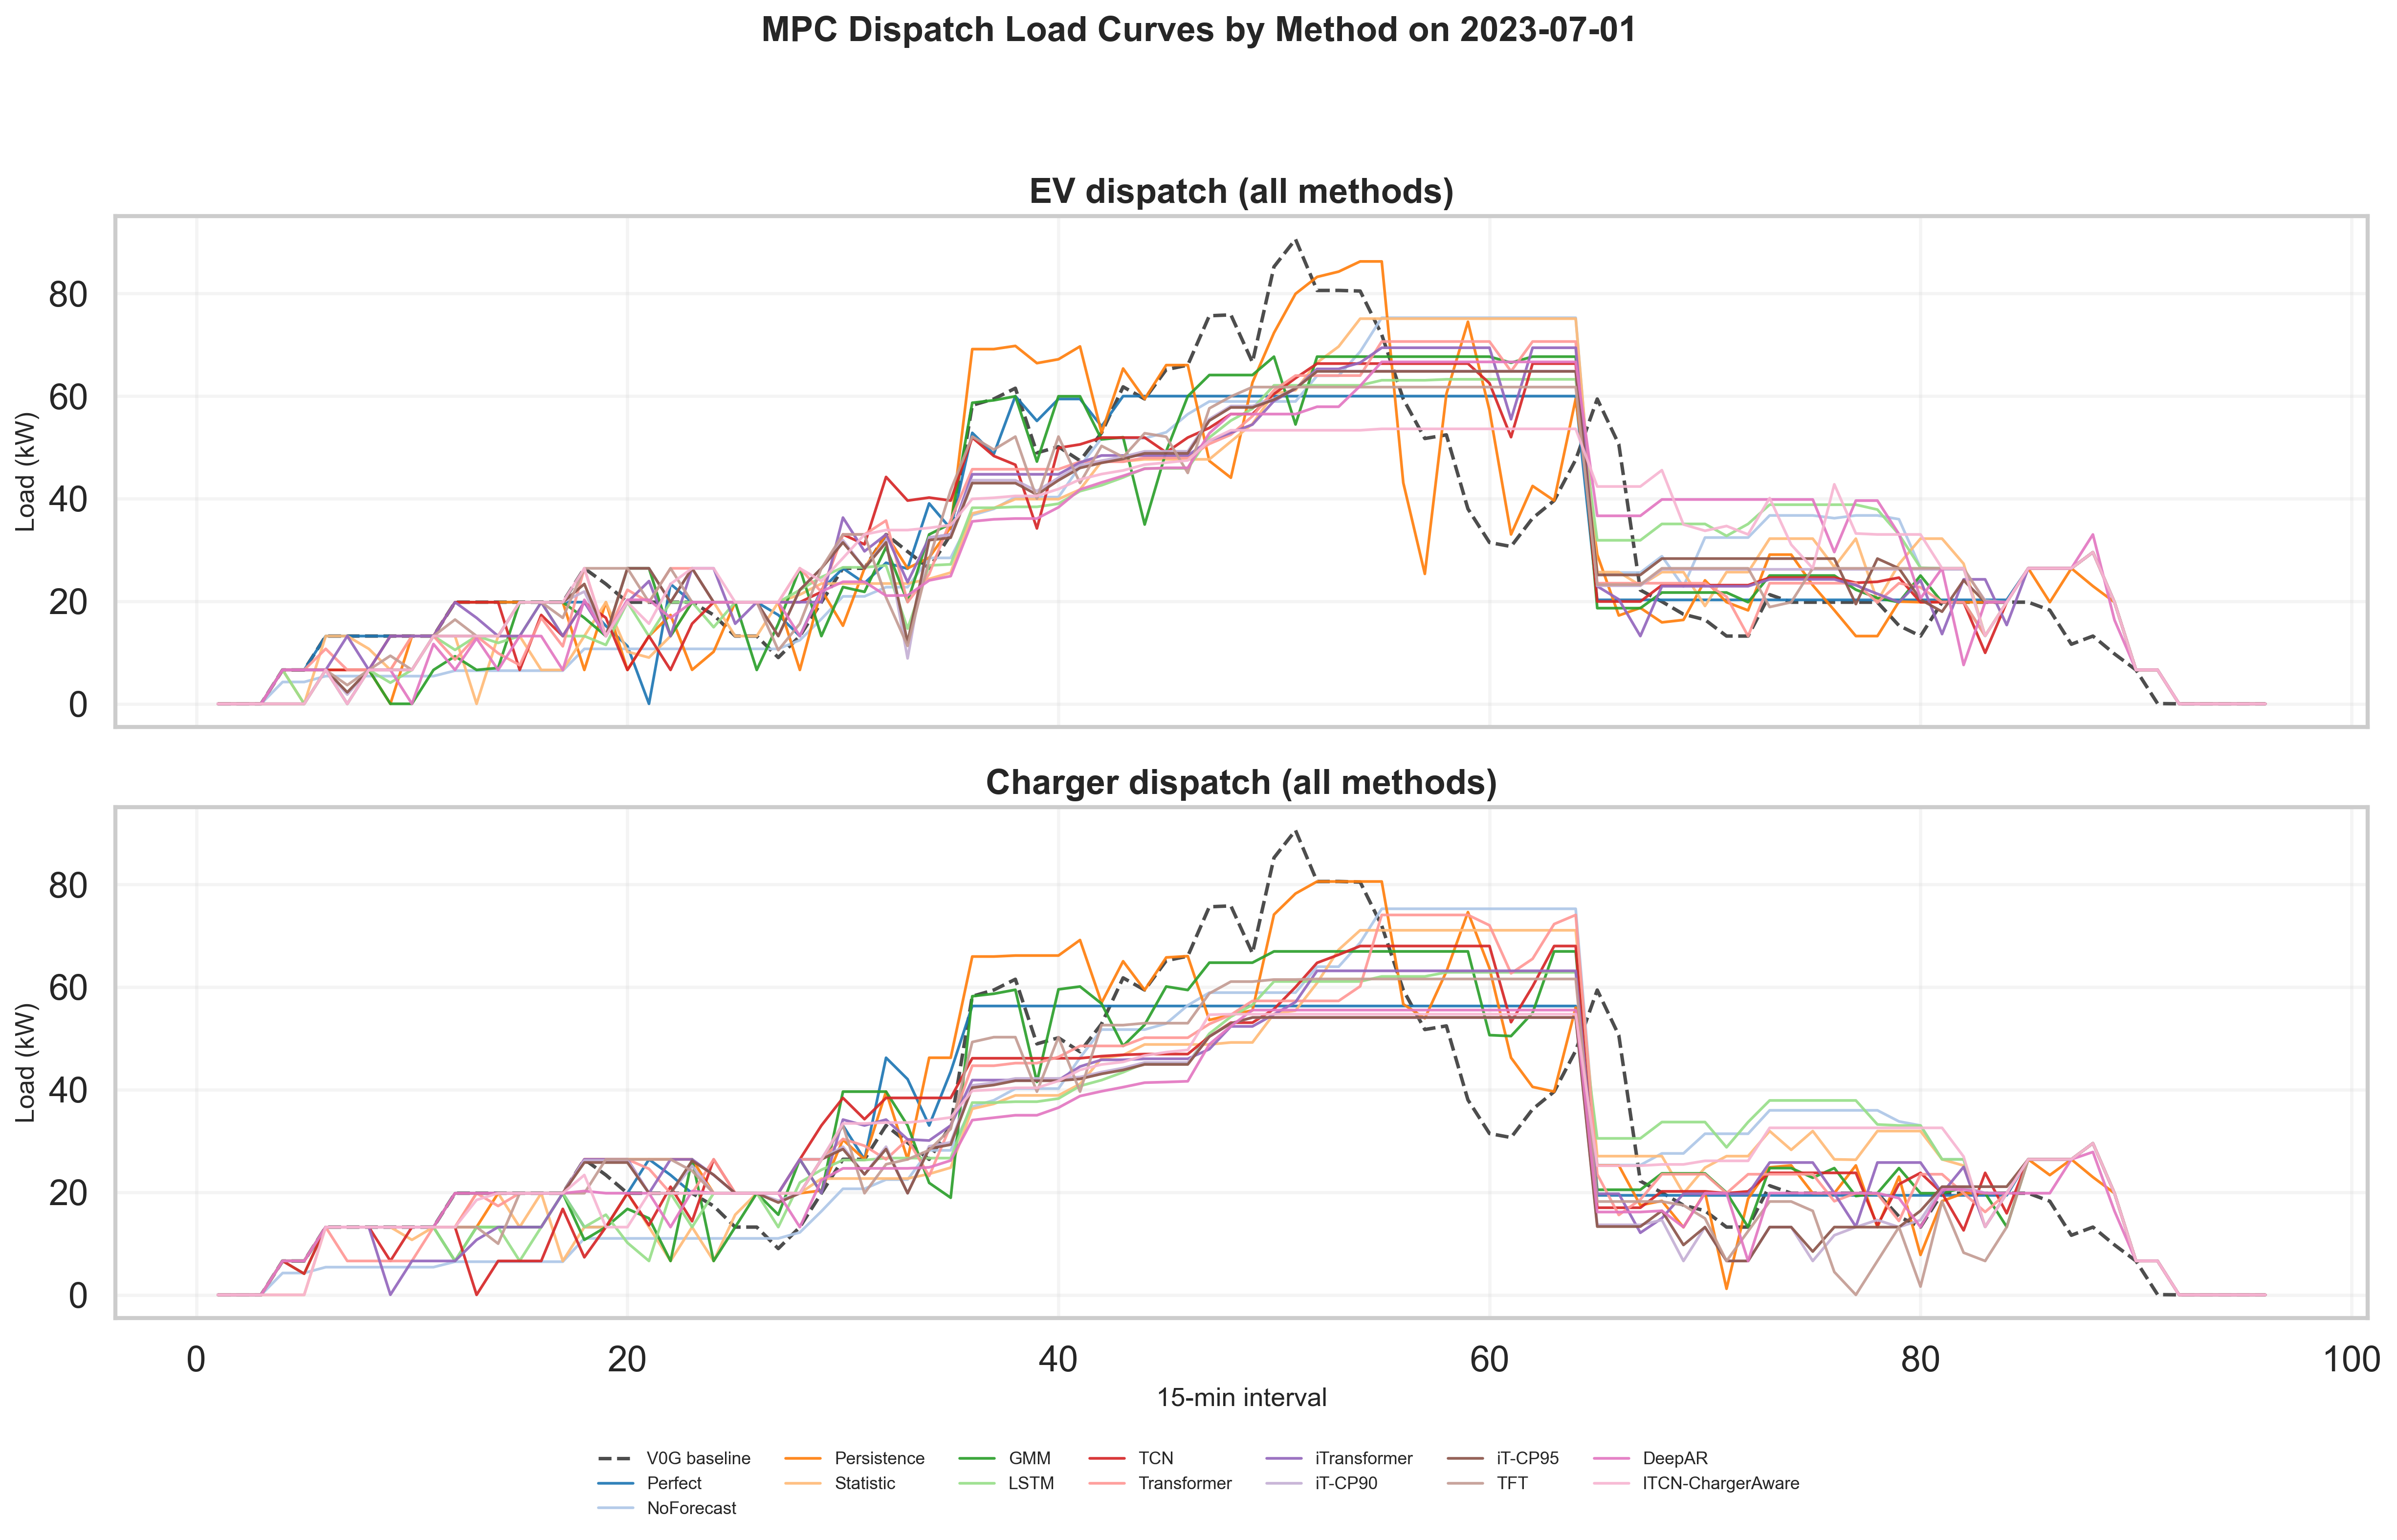
\includegraphics[width=\linewidth]{figures/0701/fig01_load_curves_all_methods.png}
\caption{MPC dispatch load curves for all methods in both cases (EV and Charger), with V0G baseline. Each colored curve is one method trajectory under a fixed MPC core.}
\label{fig:loadcurve}
\end{figure}

\begin{figure}[t]
\centering
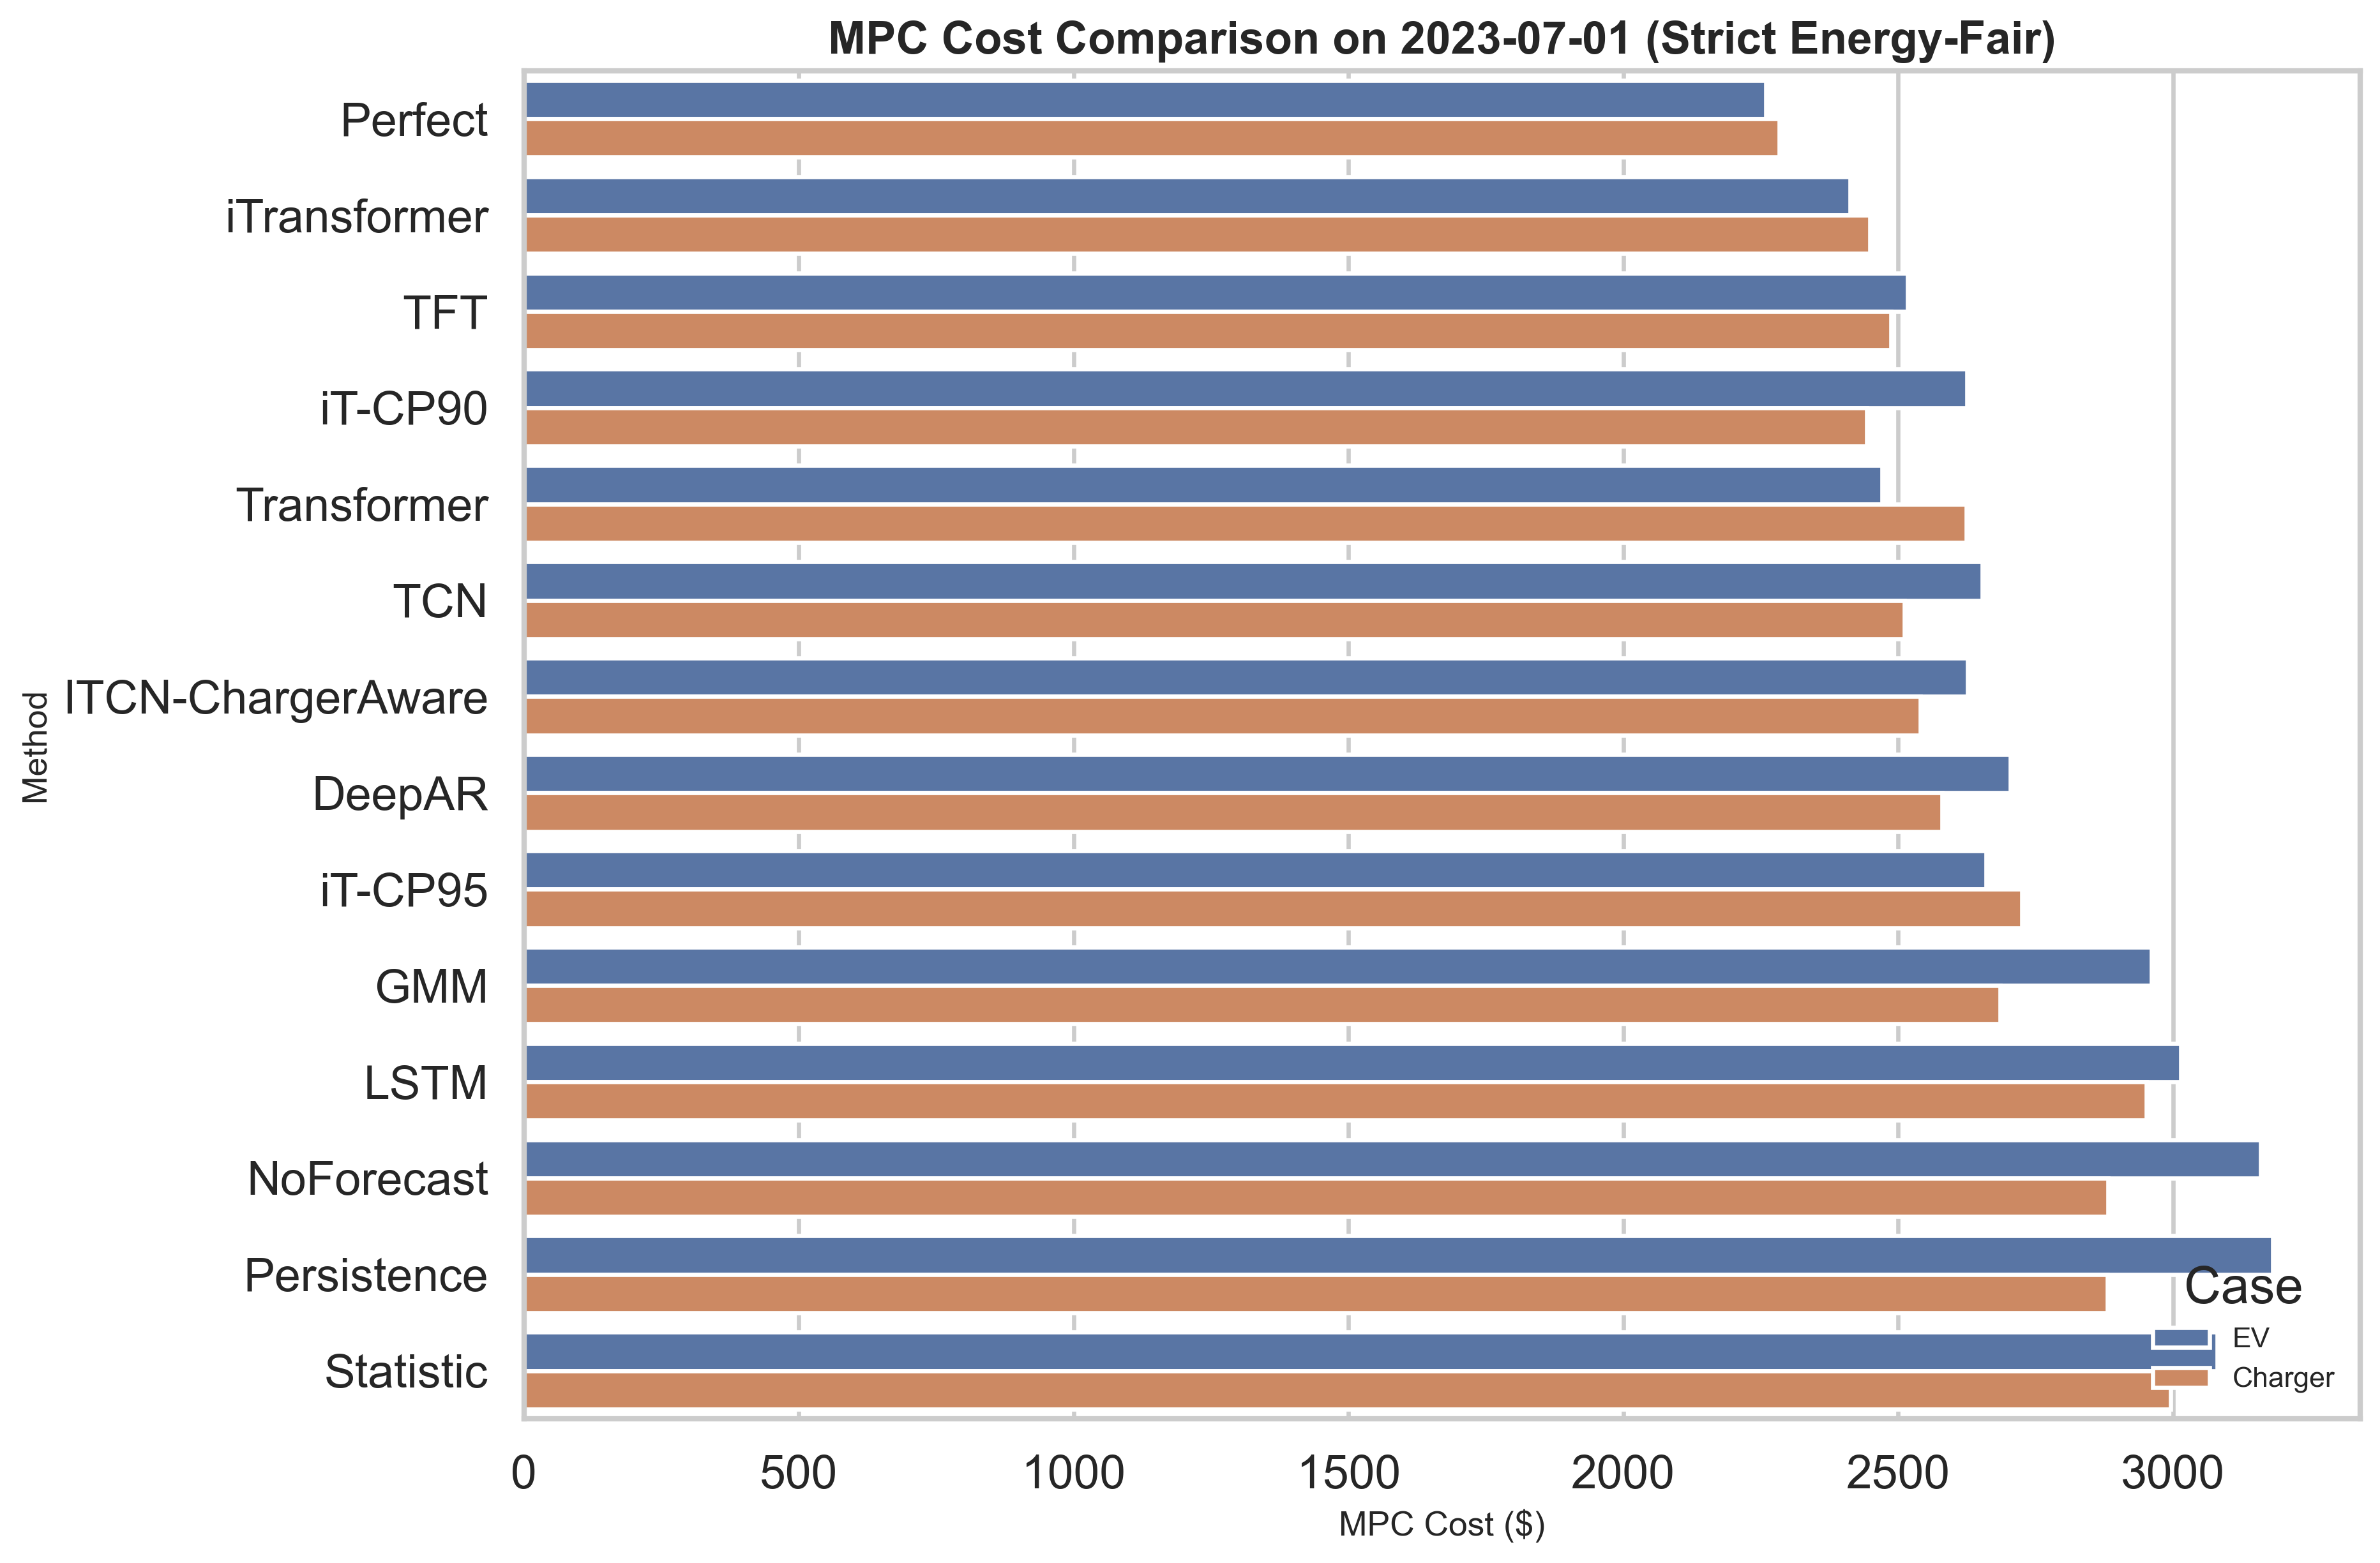
\includegraphics[width=\linewidth]{figures/0701/fig02_cost_barh.png}
\caption{Strict-fair cost comparison by method and optimization case.}
\label{fig:cost}
\end{figure}

\begin{figure}[t]
\centering
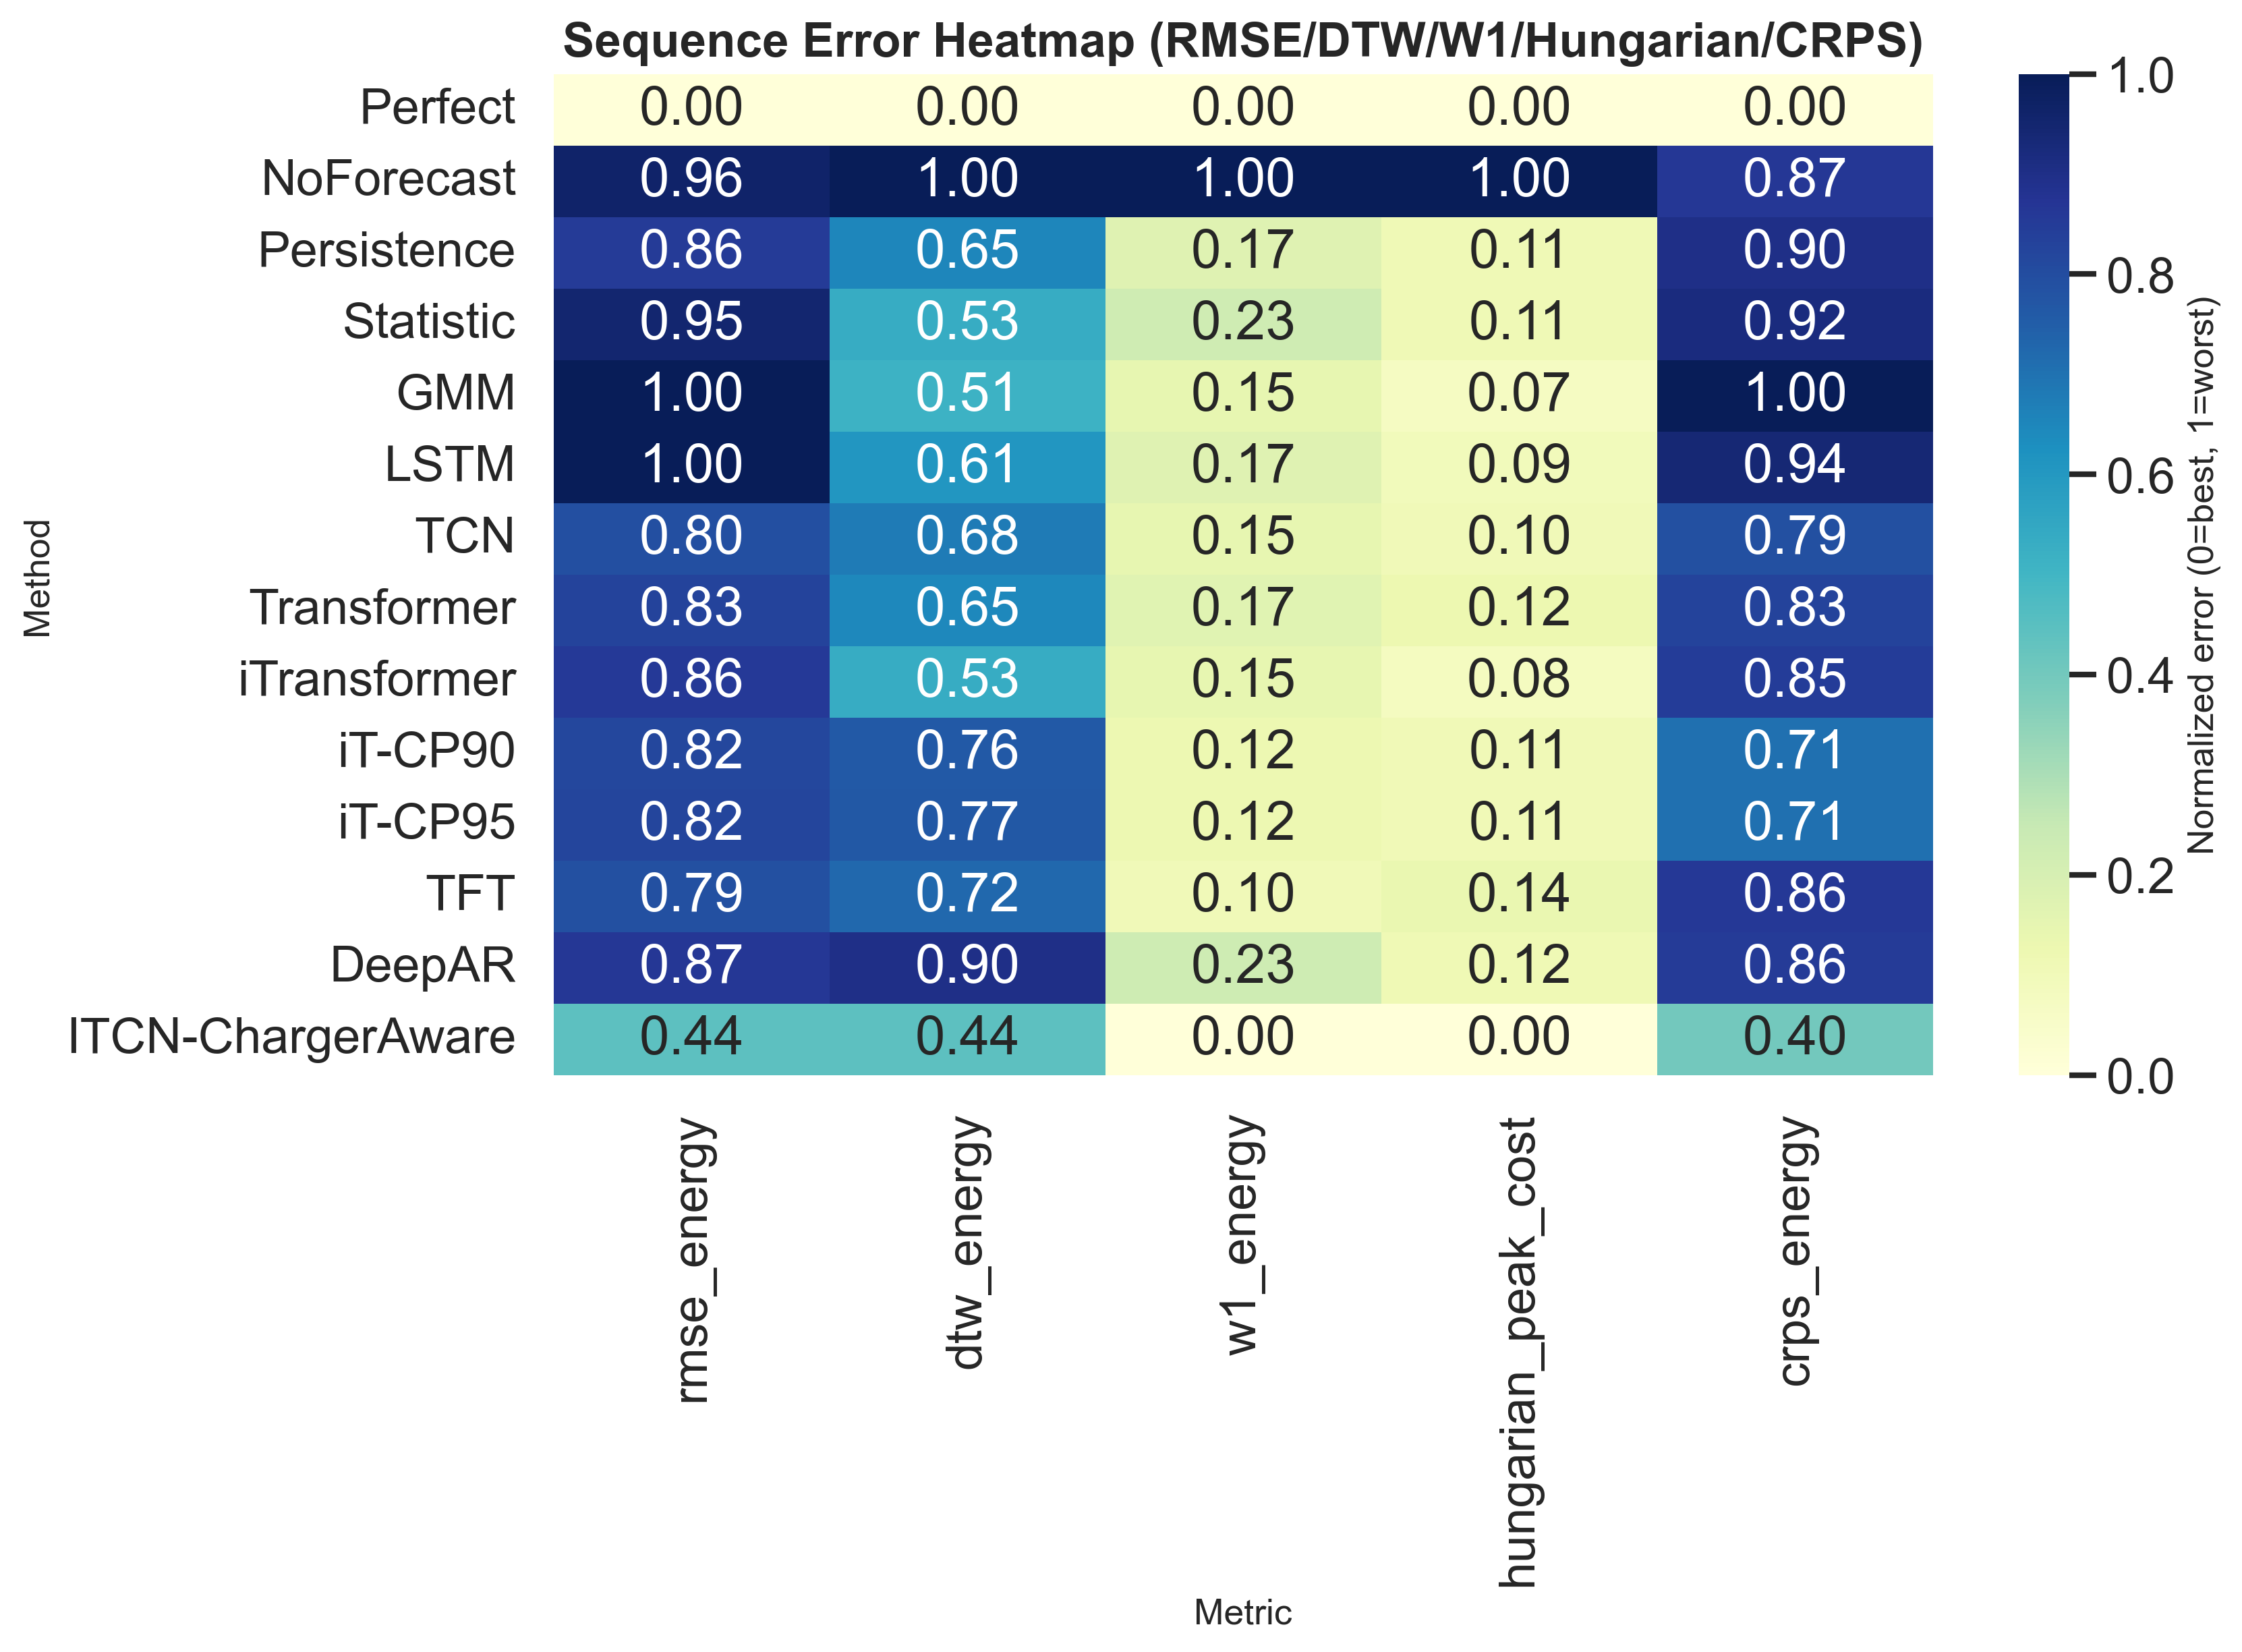
\includegraphics[width=\linewidth]{figures/0701/fig08_forecast_error_heatmap.png}
\caption{Sequence-error heatmap using RMSE, DTW, Wasserstein-$1$, Hungarian peak-assignment cost, and CRPS. Values are min-max normalized per metric (0 best, 1 worst).}
\label{fig:heatmap}
\end{figure}

\begin{figure}[t]
\centering
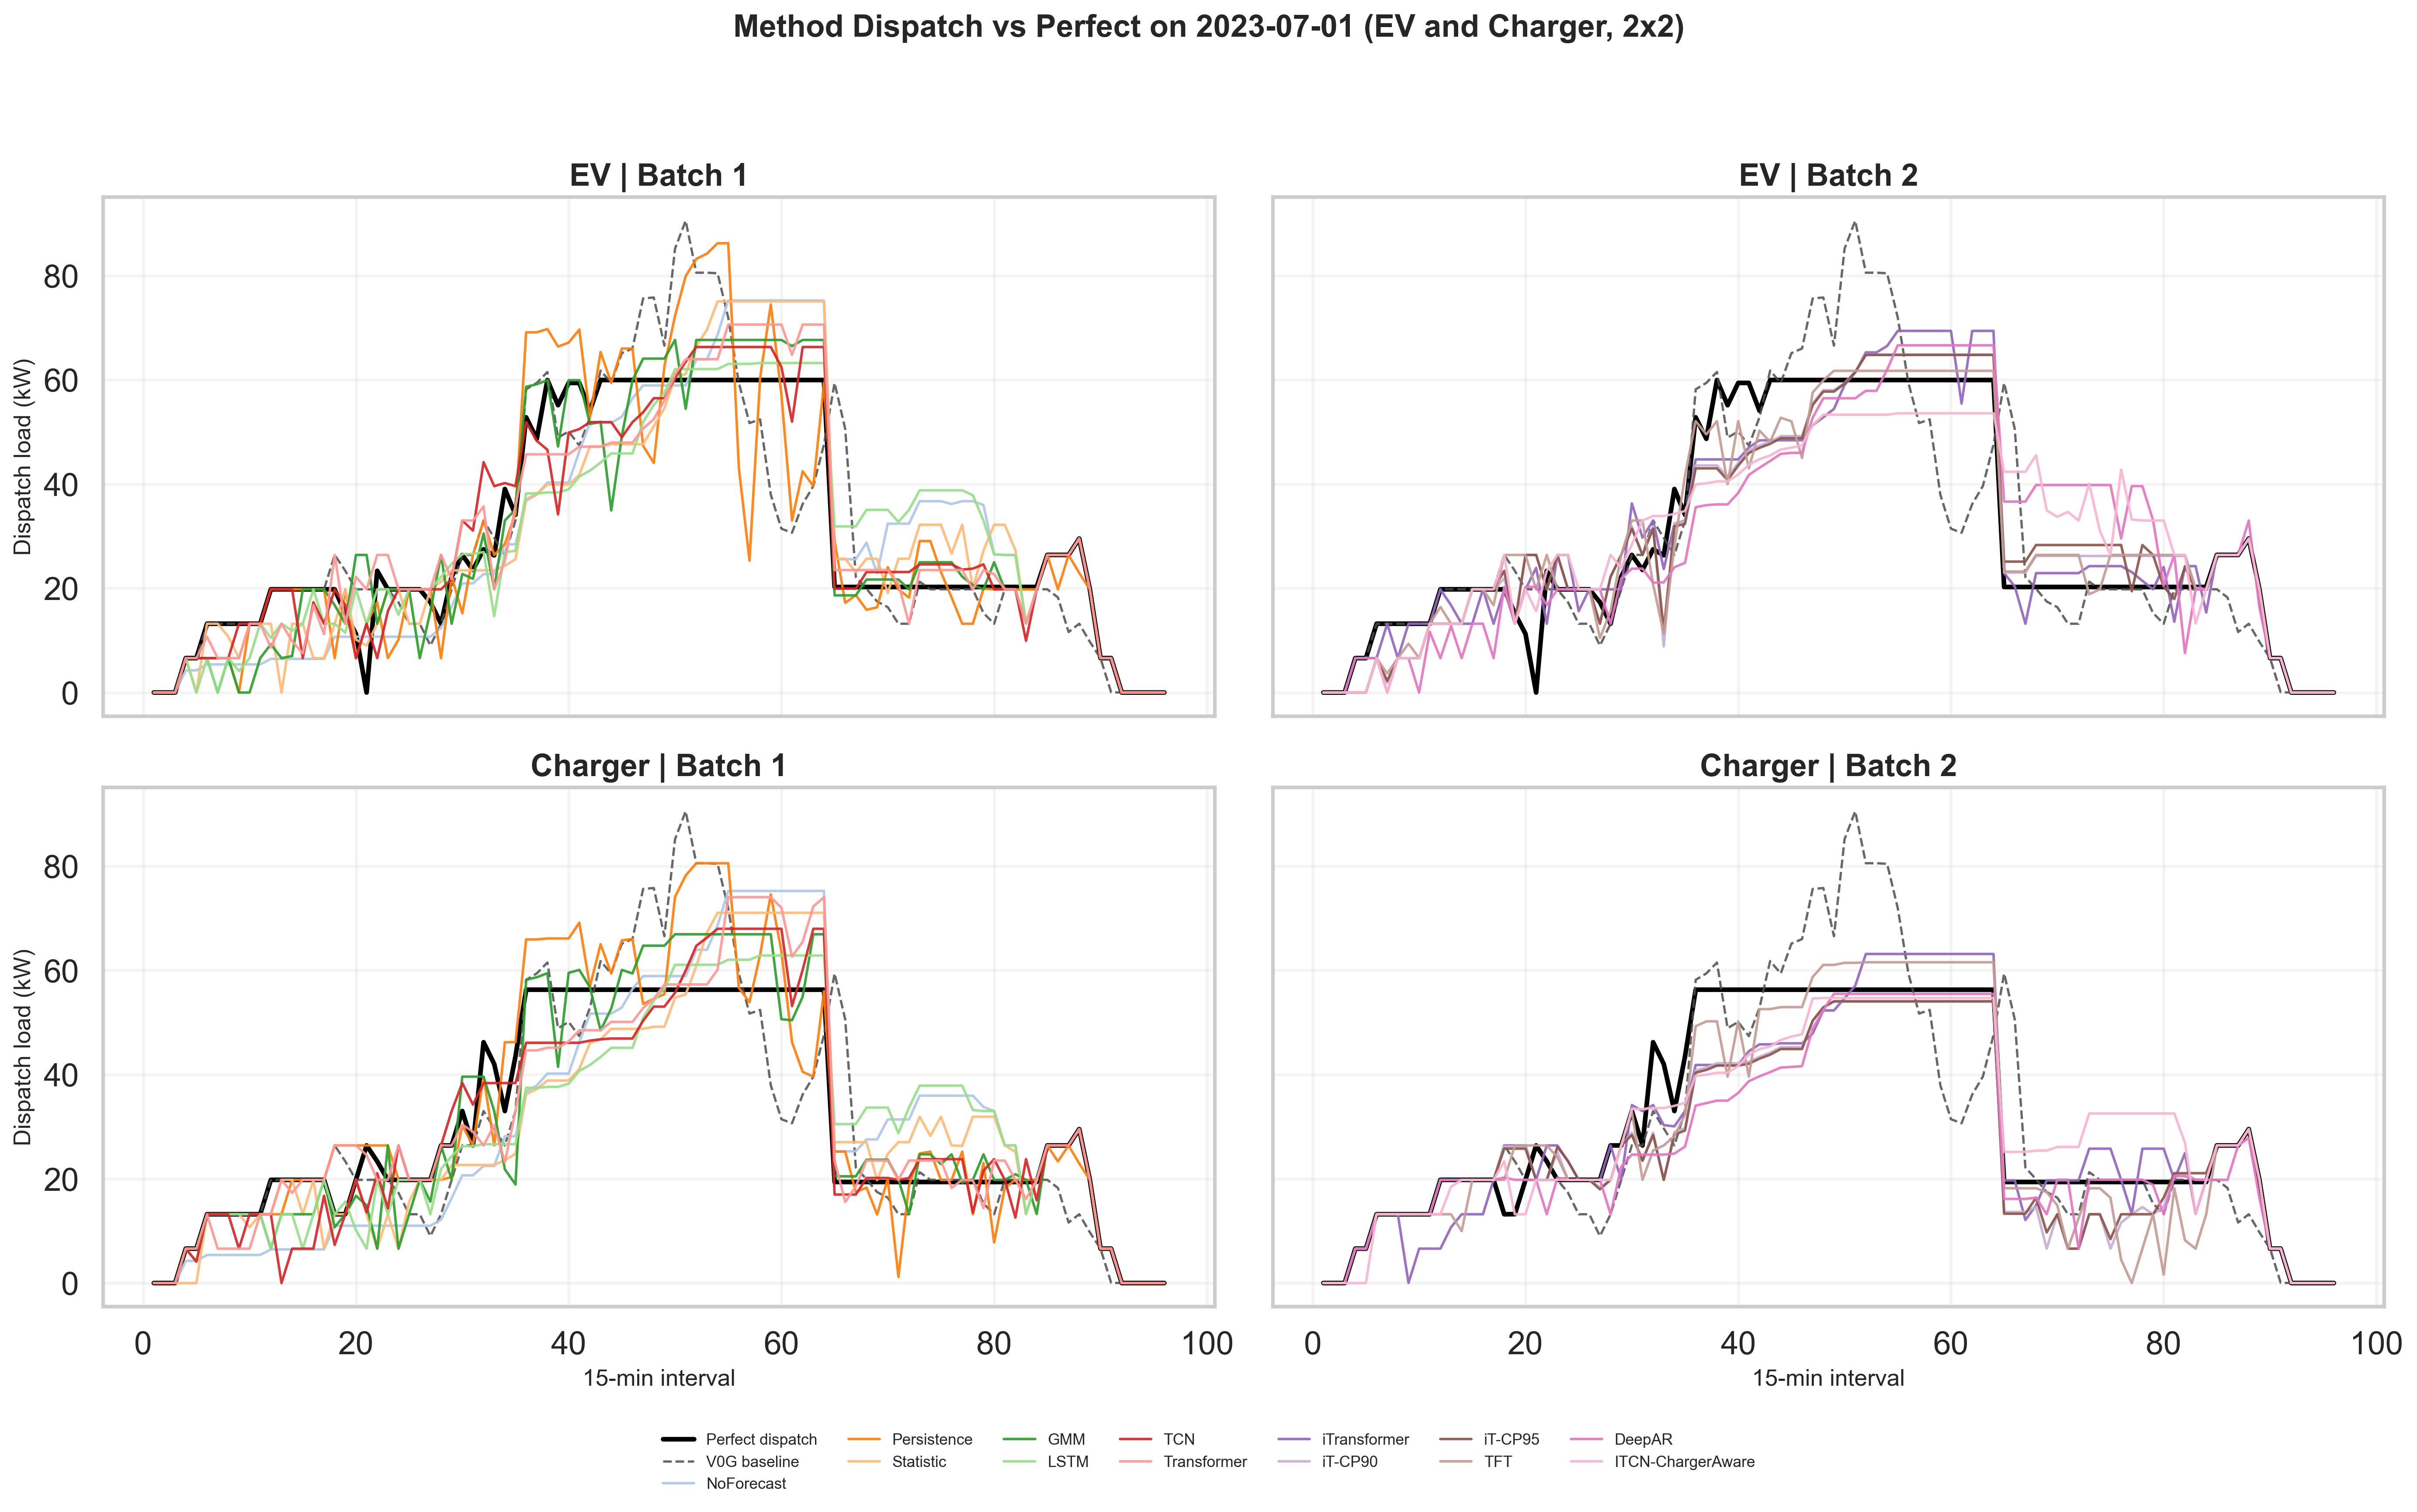
\includegraphics[width=\linewidth]{figures/0701/fig10_all_methods_vs_perfect_two_panel.png}
\caption{Forecast-driven dispatch versus perfect dispatch in a 2$\times$2 layout: rows are EV/Charger cases, columns are method batches. This figure is used to diagnose case-dependent shape distortions (especially peak-window amplification).}
\label{fig:timeseries}
\end{figure}

\begin{figure}[t]
\centering
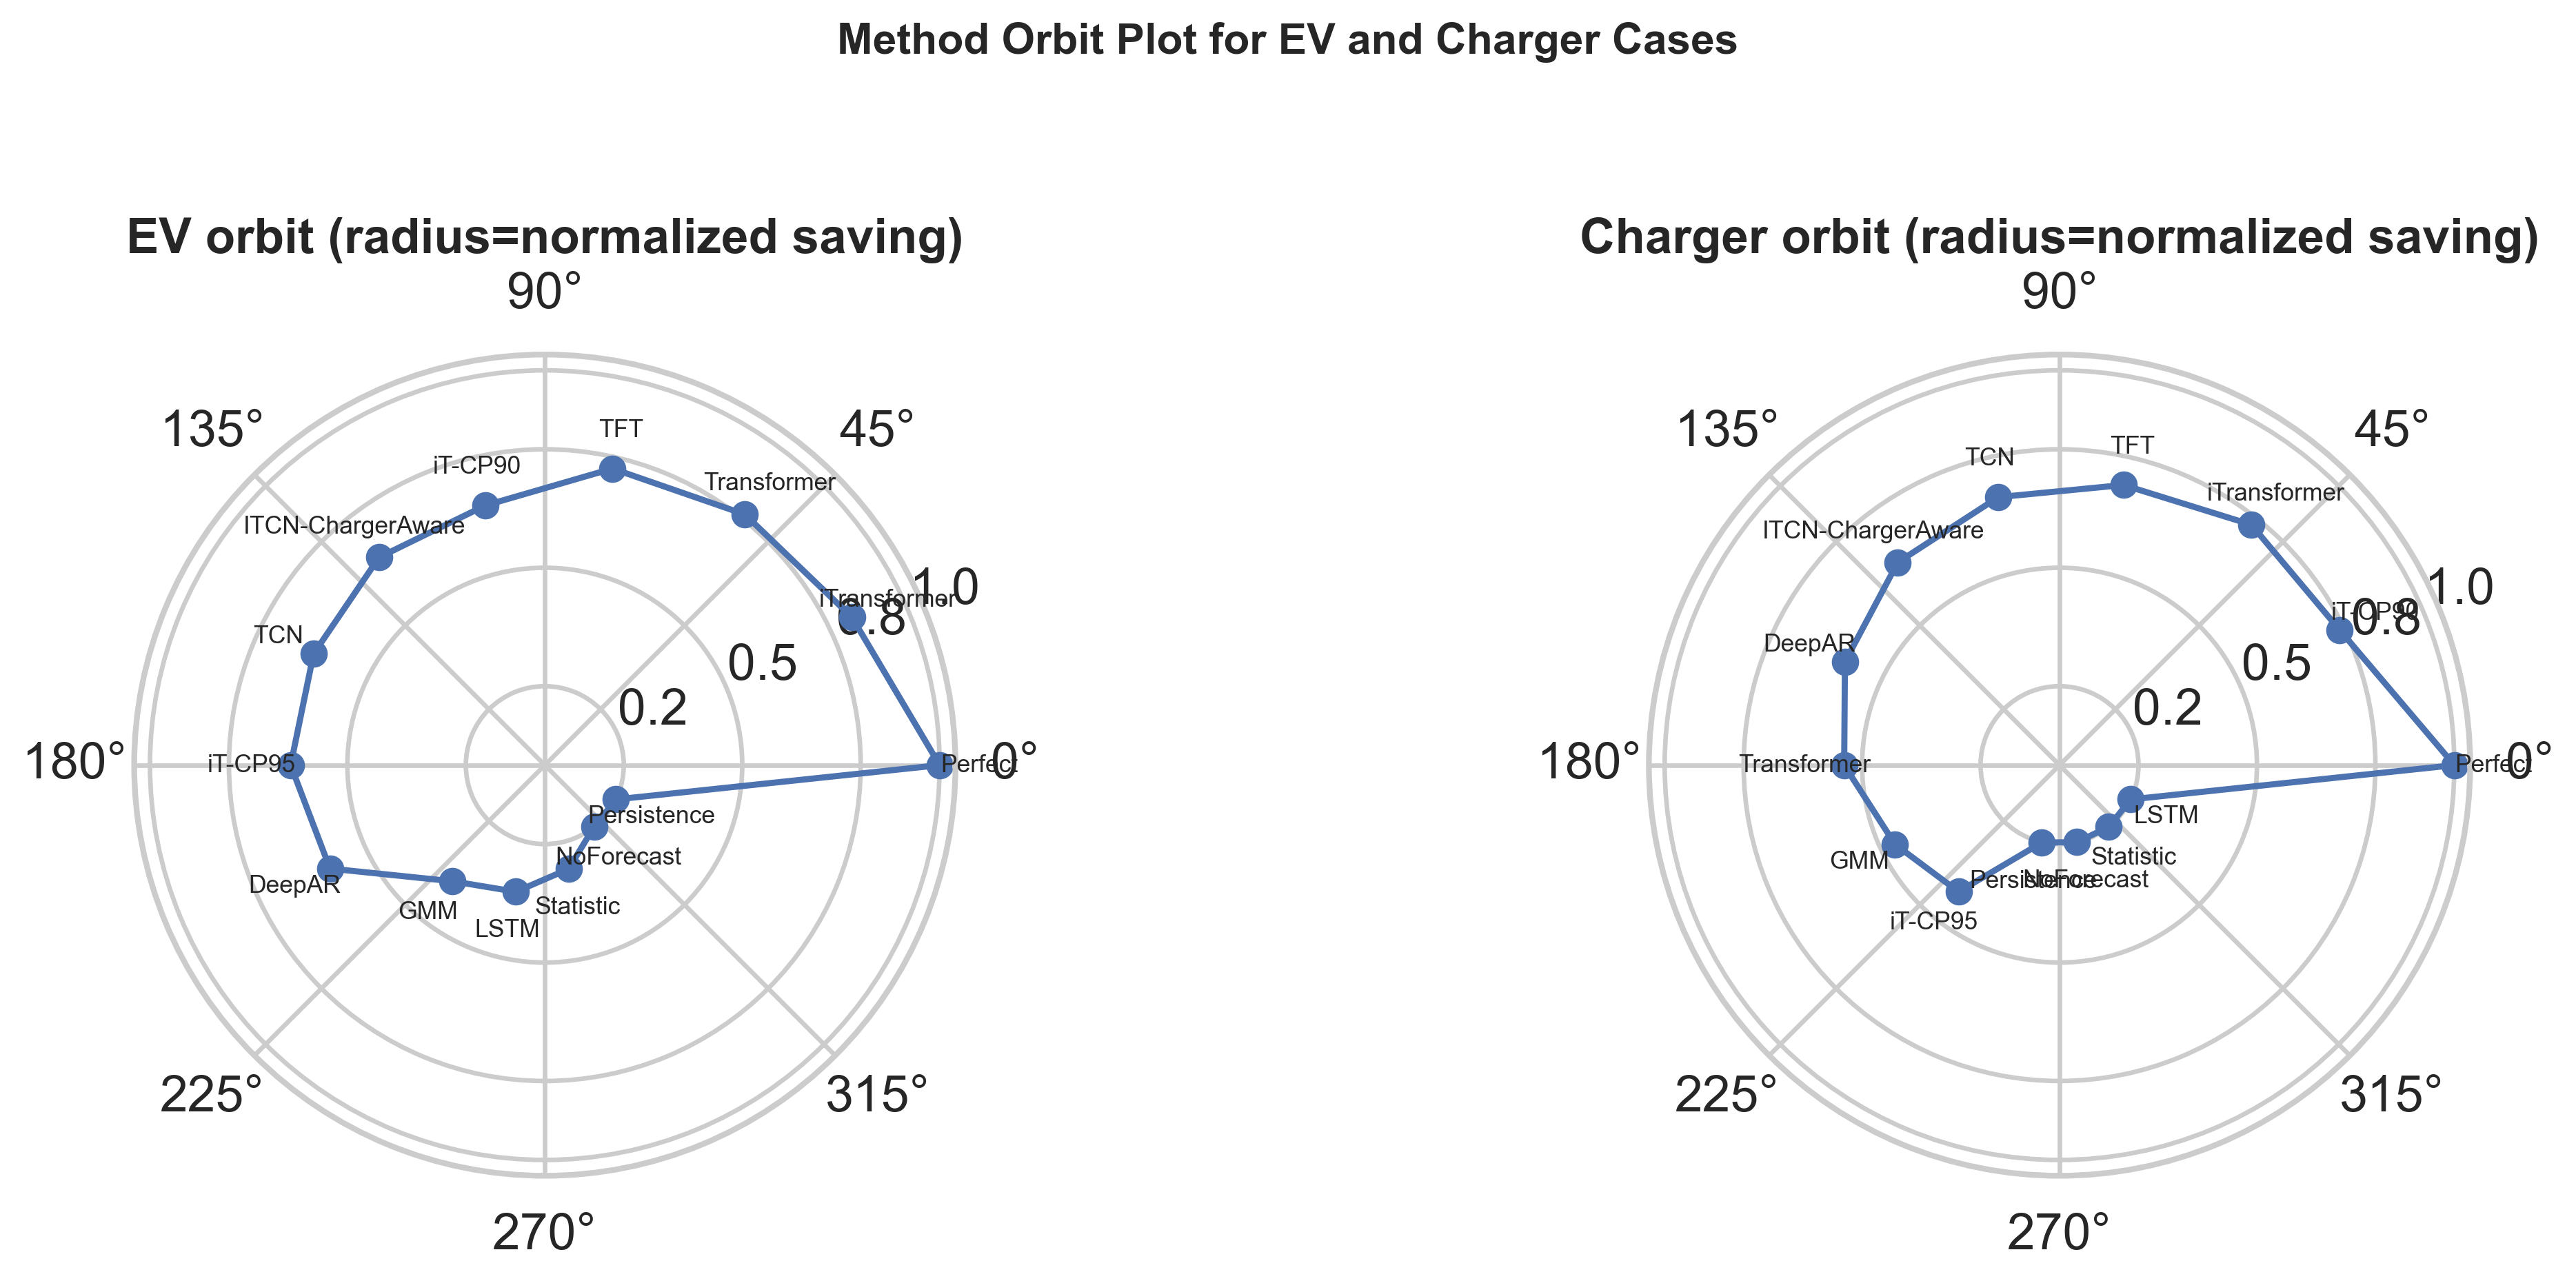
\includegraphics[width=\linewidth]{figures/0701/fig11_orbit_plot_ev_charger.png}
\caption{Orbit plot of method ranking by case. Angular coordinate indexes methods (sorted by saving); radius is normalized strict-fair saving. The EV and Charger geometry differs, indicating case-dependent ranking structure.}
\label{fig:orbit}
\end{figure}

\subsection{LP Sensitivity to Forecast Perturbation}
Our rolling model is an LP (continuous variables only; no binary on/off decision), not a MILP. Let forecast perturbation be $\delta$ and compactly write one LP step as
\begin{equation}
J^*(\delta)=\min_x\ c^\top x\quad\text{s.t.}\quad A x \ge b + B\delta,\ x\ge 0.
\end{equation}
Denote an optimal dual solution by $\lambda^*(\delta)\ge 0$. By LP duality and value-function sensitivity,
\begin{equation}
\frac{\partial J^*}{\partial \delta_j}=\lambda^{*\top}B_{:,j}
\end{equation}
for regions where active set is unchanged. Therefore, forecast error impact is weighted by dual scarcity prices of affected constraints.

A practical bound is
\begin{equation}
|J^*(\delta)-J^*(0)|\le \|\lambda^*(0)\|_{\infty}\,\|B\delta\|_1 + o(\|\delta\|),
\end{equation}
which implies: larger forecast error does not always produce larger cost degradation unless it hits high-dual-price constraints (typically near on-peak windows and deadline bottlenecks). This explains why accuracy and savings are correlated but not strictly monotone in all methods.

\subsection{Persistence vs NoForecast Diagnostic on Pilot Day}
The pilot day shows a nuanced pattern rather than a universal ordering. In EV case, NoForecast is slightly better than Persistence in strict cost (\$3158.99 vs \$3181.44), while in Charger case Persistence is slightly better than NoForecast after strict reconciliation (\$2881.01 vs \$2881.90). The main driver is peak behavior: EV-Persistence has a larger peak (\SI{85.15}{kW}) than EV-NoForecast (\SI{75.23}{kW}), consistent with over-forecasted energy (770.16 kWh forecast vs 711.19 kWh actual) increasing precautionary charging pressure.

This does \emph{not} contradict the utility of persistence-based forecasting; it indicates that a persistence prior can be harmful if the copied day is energy-heavy or temporally misaligned relative to the target day's binding tariff windows.

\subsection{Conditional Proof: Better Forecast Accuracy $\Rightarrow$ Better MPC Objective}
Define forecast error vector $e=\hat{y}-y$ for the profile components used by MPC constraints. Under fixed active set and fixed feasibility regime (no basis switch), LP sensitivity gives a local affine value function:
\begin{equation}
J^*(\hat{y})-J^*(y)=\lambda^{*\top}B e.
\end{equation}
Hence,
\begin{equation}
|J^*(\hat{y})-J^*(y)|\le L_1\|e\|_1\le L_1\sqrt{H}\|e\|_2 = L_1\sqrt{H}\,\RMSE_E,
\end{equation}
with $L_1=\|\lambda^*\|_\infty\|B\|_1$.

Consider two forecasting methods $a,b$ under the same active set neighborhood. If
\begin{equation}
\|e_a\|_2\le \|e_b\|_2
\quad\text{and}\quad
\operatorname{sign}(\lambda^{*\top}Be_a)=\operatorname{sign}(\lambda^{*\top}Be_b),
\end{equation}
then method $a$ has no larger objective deviation bound and is expected to yield no worse MPC objective locally. Therefore, for this problem class, ``better forecast gives better MPC'' is mathematically true under local regularity assumptions; globally, active-set switches can still break strict monotonic ranking.

\section{Discussion}

\subsection{Why Strict Fairness Matters}
Without energy sanity constraints, charger-level methods with larger under-delivery can appear artificially cheaper. Strict equal-energy comparison avoids this and gives reviewers a deployable ranking.

With the added NoForecast dominance guard, deployment-facing results further satisfy baseline rationality: no reported method is worse than the no-forecast controller on the same day and case.

\subsection{Forecast Accuracy vs. Control Gain}
Figures fig06, fig08, fig10, and fig11 jointly show that both timing alignment and energy profile fidelity are needed for stable control gains. The relationship is not perfectly monotone because forecast perturbations project through LP dual weights; errors on low-price slack intervals can be almost neutral, while small errors near binding windows can be expensive.

\subsection{On ``Does Better Forecast Always Mean Better Savings?''}
Not always, but usually under fixed controller and tariff. Sufficient condition for local monotonicity is that perturbations preserve active set and affect constraints with same-sign dual multipliers. Once active sets switch, value function becomes piecewise affine and ranking can change non-smoothly. Hence, we report both aggregate error metrics and optimization outcomes, rather than asserting one-to-one ordering.

\subsection{Runtime and Practicality}
The framework keeps one optimizer and swaps forecast modules, making practical deployment modular. Probabilistic methods add forecast-stage overhead but can improve robustness diagnostics. Charger-aware mapping improves implementation realism when station occupancy structure is important.

From deployment perspective, EV-level optimization is preferred when user-level control authority and communication bandwidth are available (fine-grained controllability). Charger-level optimization is preferred for backward compatibility with existing charging management systems, lower telemetry requirements, and faster solve times. The strict equal-energy wrapper is crucial when comparing these two scopes, because aggregation otherwise can appear artificially favorable through hidden under-delivery.

\subsection{Limitations and Future Methodology Extensions}
This study remains a single-day deep-dive benchmark in the strict reproducibility setting. Key extensions for a full journal campaign include:
\begin{itemize}
    \item Multi-day confidence intervals for ranking stability.
    \item Statistical tests over repeated rolling windows (e.g., paired nonparametric tests on strict-fair savings).
    \item End-to-end probabilistic MPC where forecast uncertainty is propagated directly into optimization constraints/objective.
    \item Explicit user-level fairness metrics (deadline slack distribution, tail-risk of undercharge) beyond aggregate energy equality.
\end{itemize}

\subsection{Threats to Validity}
\textbf{External validity}: pilot-day behavior may not represent seasonal variability, academic calendar effects, or infrastructure outages.\
\textbf{Model validity}: aggregate charger constraints may under-represent intra-charger heterogeneity in user deadlines.\
\textbf{Metric validity}: scalar savings alone can hide temporal-shape artifacts; therefore, sequence metrics and orbit-style geometry diagnostics are jointly reported.\
\textbf{Implementation validity}: notebook execution order or stale artifacts can introduce drift; we mitigate this via explicit manifest and strict table regeneration.

\subsection{IEEE TSG Readiness Plan}
For journal submission, we recommend the following package:
\begin{enumerate}
    \item Six-month (2024H1) day-level strict-fair tables with confidence intervals.
    \item Paired statistical tests for method comparisons in both EV and Charger cases.
    \item Ablation appendix on fairness normalization and NoForecast dominance guard impact.
    \item Reproducibility archive: notebook, tables, figure manifest, and fixed environment specifications.
\end{enumerate}
The present draft is designed to be directly extensible to that package without changing core notation or evidence chain.

\section{Reproducibility Artifact Map}
To support transparent review and replication, artifacts are organized by role:
\begin{itemize}
    \item \textbf{Modeling and execution}: \texttt{EV\_Charging\_Optimization\_Research.ipynb}
    \item \textbf{Main strict-fair results}: \texttt{tables/result\_0701\_strict\_equal\_energy.csv}
    \item \textbf{Publication table export}: \texttt{tables/publication\_main\_table.csv}
    \item \textbf{Baseline robustness audit}: \texttt{tables/noforecast\_dominance\_0701.csv}
    \item \textbf{Figure list and semantics}: \texttt{tables/figure\_manifest\_0701.csv}
    \item \textbf{Main figures}: \texttt{figures/0701/fig01\dots fig11} (without fig09 in the current version)
\end{itemize}

For reviewer convenience, each figure has an explicit core question in the manifest. This design reduces ambiguity between forecast-quality evidence and controller-output evidence.

\section{Conclusion}
This work provides a mathematically explicit and reproducible forecast-to-MPC evaluation framework with strict equal-energy fairness. The updated pipeline resolves charger under-delivery comparison bias and establishes a complete evidence chain from forecast errors to control outcomes. On the pilot day, the best non-oracle EV method is iTransformer and the best non-oracle Charger method is iT-CP90; case-level mean strict cost is lower for Charger in this pilot setting. Future work includes full six-month 2024 validation, statistical significance reporting, and end-to-end strict constraints solved directly inside rolling MPC rather than post-reconciliation.

\appendices

\section{Pilot-Day Key Parameters}
\begin{table}[h]
\caption{Core Tariff and MPC Parameters (Used in 2023-07-01 Pilot)}
\centering
\begin{tabular}{lc}
\toprule
Parameter & Value \\
\midrule
Time slots per day $H$ & 96 \\
Time-step $\Delta t$ & \SI{0.25}{h} \\
Max charging power $P_{\max}$ & \SI{6.6}{kW} \\
On-peak window & 16:00--21:00 \\
Energy price (on-peak) & \$0.126/kWh \\
Energy price (off-peak) & \$0.108/kWh \\
Demand charge (non-coincident) & \$24.48/kW \\
Additional demand charge (summer on-peak) & \$28.92/kW \\
\bottomrule
\end{tabular}
\label{tab:appendix_params}
\end{table}

\section{Additional Result Details for Persistence vs NoForecast}
\begin{table}[h]
\caption{Pilot-Day Diagnostic for Persistence and NoForecast (Strict Equal-Energy)}
\centering
\begin{tabular}{lccc}
\toprule
Method-Case & Strict Cost (\$) & Strict Saving (\%) & Peak (kW) \\
\midrule
NoForecast-EV & 3158.99 & 25.64 & 75.23 \\
Persistence-EV & 3181.44 & 25.12 & 85.15 \\
NoForecast-Charger & 2881.90 & 32.17 & 68.43 \\
Persistence-Charger & 2881.01 & 32.19 & 78.17 \\
\bottomrule
\end{tabular}
\label{tab:appendix_persistence}
\end{table}

\section{All-Method Strict Summary on Pilot Day}
\begin{table*}[t]
\caption{Full Method Comparison Under Strict Equal-Energy Normalization (2023-07-01)}
\centering
\scriptsize
\begin{tabular}{lcccccc}
\toprule
Method & EV Cost (\$) & Charger Cost (\$) & EV Saving (\%) & Charger Saving (\%) & EV Peak (kW) & Charger Peak (kW) \\
\midrule
DeepAR-Gaussian & 2704.72 & 2580.44 & 36.34 & 39.26 & 56.67 & 50.19 \\
GMM & 2960.97 & 2685.75 & 30.31 & 36.78 & 84.19 & 67.88 \\
ITCN-ChargerAware & 2626.80 & 2540.27 & 38.17 & 40.21 & 61.13 & 58.33 \\
LSTM & 3014.01 & 2881.90 & 29.06 & 32.17 & 80.09 & 72.26 \\
Noforecast & 3158.99 & 2881.90 & 25.64 & 32.17 & 75.23 & 68.43 \\
Perfect & 2259.21 & 2283.74 & 46.82 & 46.25 & 59.95 & 56.23 \\
Persistence & 3158.99 & 2881.01 & 25.64 & 32.19 & 85.15 & 78.17 \\
Statistic & 3080.43 & 2881.90 & 27.49 & 32.17 & 72.16 & 62.33 \\
TCN & 2652.90 & 2510.85 & 37.56 & 40.90 & 65.86 & 58.71 \\
TFT-Quantile & 2517.35 & 2487.21 & 40.75 & 41.46 & 65.56 & 59.02 \\
Transformer & 2470.19 & 2623.64 & 41.86 & 38.25 & 66.69 & 70.46 \\
iT-CP90 & 2624.93 & 2442.29 & 38.22 & 42.51 & 67.79 & 52.88 \\
iT-CP95 & 2659.93 & 2724.79 & 37.39 & 35.86 & 71.02 & 64.63 \\
iTransformer & 2412.99 & 2449.00 & 43.20 & 42.36 & 63.76 & 63.06 \\
\bottomrule
\end{tabular}
\label{tab:appendix_all_methods}
\end{table*}

\section*{Reproducibility Checklist}
\begin{itemize}
    \item Notebook: \texttt{EV\_Charging\_Optimization\_Research.ipynb}
    \item Strict table: \texttt{tables/result\_0701\_strict\_equal\_energy.csv}
    \item Strict sanity table: \texttt{tables/sanity\_check\_0701\_strict.csv}
    \item Sequence metric tables: \texttt{tables/timeseries\_metrics\_0701.csv}, \texttt{tables/timeseries\_metrics\_0701\_normalized.csv}
    \item Dominance audit table: \texttt{tables/noforecast\_dominance\_0701.csv}
    \item Figure manifest: \texttt{tables/figure\_manifest\_0701.csv}
    \item Sequential figures: \texttt{figures/0701/fig01\_...fig11\_...}
\end{itemize}

\bibliographystyle{IEEEtran}
\begin{thebibliography}{00}
\bibitem{mpc_ev_review}
M. Yilmaz and P. T. Krein, "Review of charging power levels and infrastructure for plug-in electric and hybrid vehicles," \emph{IEEE ISIE}, 2012.

\bibitem{tft}
B. Lim \emph{et al.}, "Temporal Fusion Transformers for interpretable multi-horizon time series forecasting," \emph{Int. J. Forecasting}, 2021.

\bibitem{deepar}
D. Salinas, V. Flunkert, J. Gasthaus, and T. Januschowski, "DeepAR: Probabilistic forecasting with autoregressive recurrent networks," \emph{Int. J. Forecasting}, 2020.

\bibitem{conformal}
Y. Romano, E. Patterson, and E. Candes, "Conformalized quantile regression," \emph{NeurIPS}, 2019.

\bibitem{transformer}
A. Vaswani \emph{et al.}, "Attention is all you need," \emph{NeurIPS}, 2017.

\bibitem{gneiting_raftery_2007}
T. Gneiting and A. E. Raftery, "Strictly proper scoring rules, prediction, and estimation," \emph{JASA}, vol. 102, no. 477, pp. 359--378, 2007.

\bibitem{dtw_sakoe}
H. Sakoe and S. Chiba, "Dynamic programming algorithm optimization for spoken word recognition," \emph{IEEE Trans. ASSP}, vol. 26, no. 1, pp. 43--49, 1978.

\bibitem{hungarian_kuhn}
H. W. Kuhn, "The Hungarian method for the assignment problem," \emph{Naval Research Logistics Quarterly}, vol. 2, pp. 83--97, 1955.
\end{thebibliography}

\end{document}
